\documentclass[twoside]{book}

% Packages required by doxygen
\usepackage{fixltx2e}
\usepackage{calc}
\usepackage{doxygen}
\usepackage[export]{adjustbox} % also loads graphicx
\usepackage{graphicx}
\usepackage[utf8]{inputenc}
\usepackage{makeidx}
\usepackage{multicol}
\usepackage{multirow}
\PassOptionsToPackage{warn}{textcomp}
\usepackage{textcomp}
\usepackage[nointegrals]{wasysym}
\usepackage[table]{xcolor}

% Font selection
\usepackage[T1]{fontenc}
\usepackage[scaled=.90]{helvet}
\usepackage{courier}
\usepackage{amssymb}
\usepackage{sectsty}
\renewcommand{\familydefault}{\sfdefault}
\allsectionsfont{%
  \fontseries{bc}\selectfont%
  \color{darkgray}%
}
\renewcommand{\DoxyLabelFont}{%
  \fontseries{bc}\selectfont%
  \color{darkgray}%
}
\newcommand{\+}{\discretionary{\mbox{\scriptsize$\hookleftarrow$}}{}{}}

% Page & text layout
\usepackage{geometry}
\geometry{%
  a4paper,%
  top=2.5cm,%
  bottom=2.5cm,%
  left=2.5cm,%
  right=2.5cm%
}
\tolerance=750
\hfuzz=15pt
\hbadness=750
\setlength{\emergencystretch}{15pt}
\setlength{\parindent}{0cm}
\setlength{\parskip}{3ex plus 2ex minus 2ex}
\makeatletter
\renewcommand{\paragraph}{%
  \@startsection{paragraph}{4}{0ex}{-1.0ex}{1.0ex}{%
    \normalfont\normalsize\bfseries\SS@parafont%
  }%
}
\renewcommand{\subparagraph}{%
  \@startsection{subparagraph}{5}{0ex}{-1.0ex}{1.0ex}{%
    \normalfont\normalsize\bfseries\SS@subparafont%
  }%
}
\makeatother

% Headers & footers
\usepackage{fancyhdr}
\pagestyle{fancyplain}
\fancyhead[LE]{\fancyplain{}{\bfseries\thepage}}
\fancyhead[CE]{\fancyplain{}{}}
\fancyhead[RE]{\fancyplain{}{\bfseries\leftmark}}
\fancyhead[LO]{\fancyplain{}{\bfseries\rightmark}}
\fancyhead[CO]{\fancyplain{}{}}
\fancyhead[RO]{\fancyplain{}{\bfseries\thepage}}
\fancyfoot[LE]{\fancyplain{}{}}
\fancyfoot[CE]{\fancyplain{}{}}
\fancyfoot[RE]{\fancyplain{}{\bfseries\scriptsize Generated by Doxygen }}
\fancyfoot[LO]{\fancyplain{}{\bfseries\scriptsize Generated by Doxygen }}
\fancyfoot[CO]{\fancyplain{}{}}
\fancyfoot[RO]{\fancyplain{}{}}
\renewcommand{\footrulewidth}{0.4pt}
\renewcommand{\chaptermark}[1]{%
  \markboth{#1}{}%
}
\renewcommand{\sectionmark}[1]{%
  \markright{\thesection\ #1}%
}

% Indices & bibliography
\usepackage{natbib}
\usepackage[titles]{tocloft}
\setcounter{tocdepth}{3}
\setcounter{secnumdepth}{5}
\makeindex

% Hyperlinks (required, but should be loaded last)
\usepackage{ifpdf}
\ifpdf
  \usepackage[pdftex,pagebackref=true]{hyperref}
\else
  \usepackage[ps2pdf,pagebackref=true]{hyperref}
\fi
\hypersetup{%
  colorlinks=true,%
  linkcolor=blue,%
  citecolor=blue,%
  unicode%
}

% Custom commands
\newcommand{\clearemptydoublepage}{%
  \newpage{\pagestyle{empty}\cleardoublepage}%
}

\usepackage{caption}
\captionsetup{labelsep=space,justification=centering,font={bf},singlelinecheck=off,skip=4pt,position=top}

%===== C O N T E N T S =====

\begin{document}

% Titlepage & ToC
\hypersetup{pageanchor=false,
             bookmarksnumbered=true,
             pdfencoding=unicode
            }
\pagenumbering{alph}
\begin{titlepage}
\vspace*{7cm}
\begin{center}%
{\Large My Project }\\
\vspace*{1cm}
{\large Generated by Doxygen 1.8.14}\\
\end{center}
\end{titlepage}
\clearemptydoublepage
\pagenumbering{roman}
\tableofcontents
\clearemptydoublepage
\pagenumbering{arabic}
\hypersetup{pageanchor=true}

%--- Begin generated contents ---
\chapter{File Index}
\section{File List}
Here is a list of all files with brief descriptions\+:\begin{DoxyCompactList}
\item\contentsline{section}{\mbox{\hyperlink{EnemyFunc_8c}{Enemy\+Func.\+c}} }{\pageref{EnemyFunc_8c}}{}
\item\contentsline{section}{\mbox{\hyperlink{GameLogic_8c}{Game\+Logic.\+c}} }{\pageref{GameLogic_8c}}{}
\item\contentsline{section}{\mbox{\hyperlink{main_8c}{main.\+c}} }{\pageref{main_8c}}{}
\item\contentsline{section}{\mbox{\hyperlink{MapFunc_8c}{Map\+Func.\+c}} }{\pageref{MapFunc_8c}}{}
\item\contentsline{section}{\mbox{\hyperlink{PlayerFunc_8c}{Player\+Func.\+c}} }{\pageref{PlayerFunc_8c}}{}
\item\contentsline{section}{\mbox{\hyperlink{Tests_8c}{Tests.\+c}} }{\pageref{Tests_8c}}{}
\item\contentsline{section}{\mbox{\hyperlink{WinManager_8c}{Win\+Manager.\+c}} }{\pageref{WinManager_8c}}{}
\end{DoxyCompactList}

\chapter{File Documentation}
\hypertarget{EnemyFunc_8c}{}\section{Enemy\+Func.\+c File Reference}
\label{EnemyFunc_8c}\index{Enemy\+Func.\+c@{Enemy\+Func.\+c}}
{\ttfamily \#include \char`\"{}Enemy\+Func.\+h\char`\"{}}\newline
Include dependency graph for Enemy\+Func.\+c\+:
\nopagebreak
\begin{figure}[H]
\begin{center}
\leavevmode
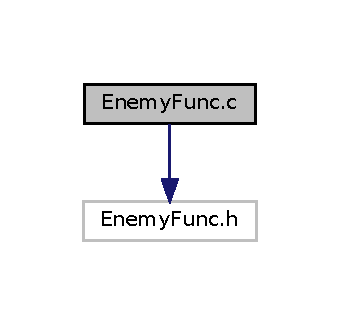
\includegraphics[width=163pt]{EnemyFunc_8c__incl}
\end{center}
\end{figure}
\subsection*{Functions}
\begin{DoxyCompactItemize}
\item 
void \mbox{\hyperlink{EnemyFunc_8c_a93990383979b8b9bf74bd8b92cb1a70d}{Initialize\+Pathfinder}} ()
\begin{DoxyCompactList}\small\item\em Função\+: Inicializa o Path\+Finder. \end{DoxyCompactList}\item 
void \mbox{\hyperlink{EnemyFunc_8c_a5a65f2b9eb6ac00383f22a01fffb93cb}{End\+Pathfinder}} ()
\begin{DoxyCompactList}\small\item\em Função\+: Finaliza o Path\+Finder. \end{DoxyCompactList}\item 
void \mbox{\hyperlink{EnemyFunc_8c_abaaae0ea27e28196515a6d59ee30e33e}{Read\+Path}} (int pathfinder\+ID, int currentX, int currentY, int pixels\+Per\+Frame)
\begin{DoxyCompactList}\small\item\em Função\+: Ler o Path. \end{DoxyCompactList}\item 
int \mbox{\hyperlink{EnemyFunc_8c_ab56151be661f2d16ed8d08ed9721c2ab}{Read\+PathX}} (int pathfinder\+ID, int \mbox{\hyperlink{EnemyFunc_8c_a47048fbd28b4f16e2075ed1500a5ce35}{path\+Location}})
\begin{DoxyCompactList}\small\item\em Função\+: Ler o Path X. \end{DoxyCompactList}\item 
int \mbox{\hyperlink{EnemyFunc_8c_a1712431bc1f9d86e24fb8362fe5434a2}{Read\+PathY}} (int pathfinder\+ID, int \mbox{\hyperlink{EnemyFunc_8c_a47048fbd28b4f16e2075ed1500a5ce35}{path\+Location}})
\begin{DoxyCompactList}\small\item\em Função\+: Ler o Path Y. \end{DoxyCompactList}\item 
void \mbox{\hyperlink{EnemyFunc_8c_a0e32ab68340fc10115bdb9cbe0361175}{move\+TroopX}} (Troop $\ast$t, int ID, int targetY, int targetX)
\begin{DoxyCompactList}\small\item\em Função\+: Mover uma Tropa do PC. \end{DoxyCompactList}\item 
void \mbox{\hyperlink{EnemyFunc_8c_a8284736a04f6600c4efca2c63f3bca04}{enemy\+Move}} (Troop $\ast$t1, Troop $\ast$t2, Troop $\ast$t3)
\begin{DoxyCompactList}\small\item\em Função\+: Controla os Movimentos do PC. \end{DoxyCompactList}\item 
void \mbox{\hyperlink{EnemyFunc_8c_aa25aa73d1953ca58dec613784df63b50}{enemy\+Troop\+Controller}} (Troop $\ast$t1, Troop $\ast$t2, Troop $\ast$t3, Build $\ast$b3, Base $\ast$b)
\begin{DoxyCompactList}\small\item\em Função\+: Controlar a Criação de Tropas do PC. \end{DoxyCompactList}\item 
void \mbox{\hyperlink{EnemyFunc_8c_ad20805e8366ccc7932aa5298a1d79ac9}{enemy\+Hit\+Control}} (Troop $\ast$t, Base $\ast$b, Build $\ast$b1, Build $\ast$b2, Build $\ast$b3)
\begin{DoxyCompactList}\small\item\em Função\+: Controlar o Ataque de Tropas do PC aos Prédios/\+Base. \end{DoxyCompactList}\item 
void \mbox{\hyperlink{EnemyFunc_8c_ae606788538ba3a44647c5629f9a2994e}{move\+Enemy\+Troop}} (Troop $\ast$t, int ID)
\begin{DoxyCompactList}\small\item\em Função\+: Mostrar Movimentos das Tropas do PC. \end{DoxyCompactList}\item 
int \mbox{\hyperlink{EnemyFunc_8c_ae730304eb738d4e118219dae2fc08683}{Find\+Path}} (int pathfinder\+ID, int startingX, int startingY, int targetX, int targetY)
\begin{DoxyCompactList}\small\item\em Função\+: Encontra um Path. \end{DoxyCompactList}\item 
int \mbox{\hyperlink{EnemyFunc_8c_a6e1ddb3286368e54f63dffc62f9a8149}{enemy\+Troop\+Checker}} (Troop $\ast$t, int mode)
\begin{DoxyCompactList}\small\item\em Função\+: Verificar as Redondezas da Tropa do PC. \end{DoxyCompactList}\end{DoxyCompactItemize}
\subsection*{Variables}
\begin{DoxyCompactItemize}
\item 
Base \mbox{\hyperlink{EnemyFunc_8c_a5f1823c63772e3cb26f42bf3de7d1ffb}{Base\+\_\+e}}
\item 
Build \mbox{\hyperlink{EnemyFunc_8c_a3fdbc37eb9f14d40fe63b611633f8df1}{B1\+\_\+e}}
\item 
Build \mbox{\hyperlink{EnemyFunc_8c_abbe13ddd2be6b6adced0e509780d02e2}{B2\+\_\+e}}
\item 
Build \mbox{\hyperlink{EnemyFunc_8c_ae2f45c6f02db7c8ab0fcfb05a8adc1dc}{B3\+\_\+e}}
\item 
Troop \mbox{\hyperlink{EnemyFunc_8c_a2e00c7c94e8a81cc896bce8956a9a032}{T1\+\_\+e}}
\item 
Troop \mbox{\hyperlink{EnemyFunc_8c_aea29d96d5040789995c1e03e8faaa1f9}{T2\+\_\+e}}
\item 
Troop \mbox{\hyperlink{EnemyFunc_8c_acb6791b0f5d4c21d96ed588ece080e38}{T3\+\_\+e}}
\item 
int \mbox{\hyperlink{EnemyFunc_8c_a6075c92d97c21a49ef8db637371c434a}{not\+Started}} = 0
\item 
int \mbox{\hyperlink{EnemyFunc_8c_ac6c6cd839d50c91230f55ed55d0cd635}{found}} = 1
\item 
int \mbox{\hyperlink{EnemyFunc_8c_ae4684897fd37cdf40aaa7e1a9737dac2}{nonexistent}} = 2
\item 
int \mbox{\hyperlink{EnemyFunc_8c_a49efc706b17c89b3843c99c488ef1f0e}{walkable}} = 0
\item 
int \mbox{\hyperlink{EnemyFunc_8c_a5229b2af98af6c573c548b257f4a5eae}{unwalkable}} = 1
\item 
int \mbox{\hyperlink{EnemyFunc_8c_ab30aaad137fac858bc09cd595a0e4db7}{number\+People}} = 3
\item 
int $\ast$ \mbox{\hyperlink{EnemyFunc_8c_a347ae6c1c2b341b6d2d92bf36d78efaa}{path\+Bank}} \mbox{[}4\mbox{]}
\item 
int \mbox{\hyperlink{EnemyFunc_8c_a742dca0a31ff8eb481bf1167597edfcf}{path\+Length}} \mbox{[}4\mbox{]}
\item 
int \mbox{\hyperlink{EnemyFunc_8c_a4133acb1b6a57058b57218646b115702}{path\+Status}} \mbox{[}4\mbox{]}
\item 
int \mbox{\hyperlink{EnemyFunc_8c_a47048fbd28b4f16e2075ed1500a5ce35}{path\+Location}} \mbox{[}4\mbox{]}
\item 
int \mbox{\hyperlink{EnemyFunc_8c_a7bce088cbd7712e387f5a341410fb0e4}{x\+Path}} \mbox{[}4\mbox{]}
\item 
int \mbox{\hyperlink{EnemyFunc_8c_a7c2f5bf65183a339ea02ad6966ae0a72}{y\+Path}} \mbox{[}4\mbox{]}
\end{DoxyCompactItemize}


\subsection{Function Documentation}
\mbox{\Hypertarget{EnemyFunc_8c_a5a65f2b9eb6ac00383f22a01fffb93cb}\label{EnemyFunc_8c_a5a65f2b9eb6ac00383f22a01fffb93cb}} 
\index{Enemy\+Func.\+c@{Enemy\+Func.\+c}!End\+Pathfinder@{End\+Pathfinder}}
\index{End\+Pathfinder@{End\+Pathfinder}!Enemy\+Func.\+c@{Enemy\+Func.\+c}}
\subsubsection{\texorpdfstring{End\+Pathfinder()}{EndPathfinder()}}
{\footnotesize\ttfamily void End\+Pathfinder (\begin{DoxyParamCaption}{ }\end{DoxyParamCaption})}



Função\+: Finaliza o Path\+Finder. 

Descrição\+: A Função desaloca a memória usada pelo Pathfinder.

Parâmetros\+: 
\begin{DoxyParams}{Parameters}
{\em Sem} & Parâmetros\\
\hline
\end{DoxyParams}
Valor retornado\+: \begin{DoxyReturn}{Returns}
Void -\/ A função não retorna nada
\end{DoxyReturn}
Assertiva de entrada\+: Sem parâmetros

Assertiva de saída\+: Função Void \mbox{\Hypertarget{EnemyFunc_8c_ad20805e8366ccc7932aa5298a1d79ac9}\label{EnemyFunc_8c_ad20805e8366ccc7932aa5298a1d79ac9}} 
\index{Enemy\+Func.\+c@{Enemy\+Func.\+c}!enemy\+Hit\+Control@{enemy\+Hit\+Control}}
\index{enemy\+Hit\+Control@{enemy\+Hit\+Control}!Enemy\+Func.\+c@{Enemy\+Func.\+c}}
\subsubsection{\texorpdfstring{enemy\+Hit\+Control()}{enemyHitControl()}}
{\footnotesize\ttfamily void enemy\+Hit\+Control (\begin{DoxyParamCaption}\item[{Troop $\ast$}]{t,  }\item[{Base $\ast$}]{b,  }\item[{Build $\ast$}]{b1,  }\item[{Build $\ast$}]{b2,  }\item[{Build $\ast$}]{b3 }\end{DoxyParamCaption})}



Função\+: Controlar o Ataque de Tropas do PC aos Prédios/\+Base. 

Descrição\+: A Função recebe as structs dos prédios, da base e de uma tropa. Ela verifica se a tropa está perto de algum prédio/base e se estiver é calculado o dano que essa tropa está dando no prédio/base. Antes de diminuir a vida do prédio/base é necessário diminuir a defesa para 0.

Parâmetros\+: 
\begin{DoxyParams}{Parameters}
{\em Troop$\ast$} & t -\/ struct da tropa do tipo 1 do PC \\
\hline
{\em Base$\ast$} & b -\/ struct da base \\
\hline
{\em Build$\ast$} & b1 -\/ struct do prédio do tipo 1 \\
\hline
{\em Build$\ast$} & b2 -\/ struct do prédio do tipo 2 \\
\hline
{\em Build$\ast$} & b3 -\/ struct do prédio do tipo 3\\
\hline
\end{DoxyParams}
Valor retornado\+: \begin{DoxyReturn}{Returns}
Void. A função não retorna nada
\end{DoxyReturn}
Assertiva de entrada\+: Troop$\ast$ t != N\+U\+LL Base$\ast$ b != N\+U\+LL Build$\ast$ b1 != N\+U\+LL Build$\ast$ b2 != N\+U\+LL Build$\ast$ b3 != N\+U\+LL

Assertiva de saída\+: Função void \mbox{\Hypertarget{EnemyFunc_8c_a8284736a04f6600c4efca2c63f3bca04}\label{EnemyFunc_8c_a8284736a04f6600c4efca2c63f3bca04}} 
\index{Enemy\+Func.\+c@{Enemy\+Func.\+c}!enemy\+Move@{enemy\+Move}}
\index{enemy\+Move@{enemy\+Move}!Enemy\+Func.\+c@{Enemy\+Func.\+c}}
\subsubsection{\texorpdfstring{enemy\+Move()}{enemyMove()}}
{\footnotesize\ttfamily void enemy\+Move (\begin{DoxyParamCaption}\item[{Troop $\ast$}]{t1,  }\item[{Troop $\ast$}]{t2,  }\item[{Troop $\ast$}]{t3 }\end{DoxyParamCaption})}



Função\+: Controla os Movimentos do PC. 

Descrição\+: A Função inicia a procura de paths e chama uma função de mover as tropas.

Parâmetros\+: 
\begin{DoxyParams}{Parameters}
{\em Troop$\ast$} & t1 -\/ Tropa do tipo 1 do PC \\
\hline
{\em Troop$\ast$} & t2 -\/ Tropa do tipo 2 do PC \\
\hline
{\em Troop$\ast$} & t3 -\/ Tropa do tipo 3 do PC\\
\hline
\end{DoxyParams}
Valor retornado\+: \begin{DoxyReturn}{Returns}
Void -\/ A Função não retorna nada
\end{DoxyReturn}
Assertiva de entrada\+: Troop$\ast$ t1 != N\+U\+LL Troop$\ast$ t2 != N\+U\+LL Troop$\ast$ t3 != N\+U\+LL

Assertiva de saída\+: Função Void \mbox{\Hypertarget{EnemyFunc_8c_a6e1ddb3286368e54f63dffc62f9a8149}\label{EnemyFunc_8c_a6e1ddb3286368e54f63dffc62f9a8149}} 
\index{Enemy\+Func.\+c@{Enemy\+Func.\+c}!enemy\+Troop\+Checker@{enemy\+Troop\+Checker}}
\index{enemy\+Troop\+Checker@{enemy\+Troop\+Checker}!Enemy\+Func.\+c@{Enemy\+Func.\+c}}
\subsubsection{\texorpdfstring{enemy\+Troop\+Checker()}{enemyTroopChecker()}}
{\footnotesize\ttfamily int enemy\+Troop\+Checker (\begin{DoxyParamCaption}\item[{Troop $\ast$}]{t,  }\item[{int}]{mode }\end{DoxyParamCaption})}



Função\+: Verificar as Redondezas da Tropa do PC. 

Descrição\+: A Função recebe a struct de uma tropa e verifica as redondezas dessa tropa, e retorna um valor de acordo com o que está do lado dessa tropa.

Parâmetros\+: 
\begin{DoxyParams}{Parameters}
{\em Troop$\ast$} & t -\/ struct da tropa \\
\hline
{\em int} & mode -\/ flag para identificar se a função foi chamada para checar se a tropa está perto do prédio responsável por aumentar tropas (0) ou se foi chamada para checar se há tropas inimigas por perto (1)\\
\hline
\end{DoxyParams}
Valor retornado\+: \begin{DoxyReturn}{Returns}
0 -\/ caso a tropa não esteja perto de nada 

1 -\/ caso a mode = 0 e a tropa esteja perto do prédio responsável por gerar tropas 

4 -\/ caso a tropa esteja perto do base \textquotesingle{}B\textquotesingle{} 

5 -\/ caso a tropa esteja perto do prédio \textquotesingle{}X\textquotesingle{} 

6 -\/ caso a tropa esteja perto do prédio \textquotesingle{}Y\textquotesingle{} 

7 -\/ caso a tropa esteja perto do prédio \textquotesingle{}Z\textquotesingle{}
\end{DoxyReturn}
Assertiva de entrada\+: Troop$\ast$ t != N\+U\+LL int mode == 0 $\vert$$\vert$ mode == 1

Assertiva de saída\+: A função retorna valores fixos. \mbox{\Hypertarget{EnemyFunc_8c_aa25aa73d1953ca58dec613784df63b50}\label{EnemyFunc_8c_aa25aa73d1953ca58dec613784df63b50}} 
\index{Enemy\+Func.\+c@{Enemy\+Func.\+c}!enemy\+Troop\+Controller@{enemy\+Troop\+Controller}}
\index{enemy\+Troop\+Controller@{enemy\+Troop\+Controller}!Enemy\+Func.\+c@{Enemy\+Func.\+c}}
\subsubsection{\texorpdfstring{enemy\+Troop\+Controller()}{enemyTroopController()}}
{\footnotesize\ttfamily void enemy\+Troop\+Controller (\begin{DoxyParamCaption}\item[{Troop $\ast$}]{t1,  }\item[{Troop $\ast$}]{t2,  }\item[{Troop $\ast$}]{t3,  }\item[{Build $\ast$}]{b3,  }\item[{Base $\ast$}]{b }\end{DoxyParamCaption})}



Função\+: Controlar a Criação de Tropas do PC. 

Descrição\+: A Função recebe as structs da base, das tropas e do prédio responsável pela criação de tropas. Então ela verifica se a tropa está do lado do prédio que gera tropa, e se há recursos para gerar mais tropas. Então essa tropa tem a quantidade aumentada.

Parâmetros\+: 
\begin{DoxyParams}{Parameters}
{\em Troop$\ast$} & t1 -\/ struct da tropa do tipo 1 do PC \\
\hline
{\em Troop$\ast$} & t2 -\/ struct da tropa do tipo 2 do PC \\
\hline
{\em Troop$\ast$} & t3 -\/ struct da tropa do tipo 3 do PC \\
\hline
{\em Build$\ast$} & b3 -\/ struct do prédio do tipo 3 do PC \\
\hline
{\em Base$\ast$} & b -\/ struct da base do PC\\
\hline
\end{DoxyParams}
Valor retornado\+: \begin{DoxyReturn}{Returns}
Void. A função não retorna nada
\end{DoxyReturn}
Assertiva de entrada\+: Troop$\ast$ t1 != N\+U\+LL Troop$\ast$ t2 != N\+U\+LL Troop$\ast$ t3 != N\+U\+LL Build$\ast$ b3 != N\+U\+LL Base$\ast$ b != N\+U\+LL

Assertiva de saída\+: Função void \mbox{\Hypertarget{EnemyFunc_8c_ae730304eb738d4e118219dae2fc08683}\label{EnemyFunc_8c_ae730304eb738d4e118219dae2fc08683}} 
\index{Enemy\+Func.\+c@{Enemy\+Func.\+c}!Find\+Path@{Find\+Path}}
\index{Find\+Path@{Find\+Path}!Enemy\+Func.\+c@{Enemy\+Func.\+c}}
\subsubsection{\texorpdfstring{Find\+Path()}{FindPath()}}
{\footnotesize\ttfamily int Find\+Path (\begin{DoxyParamCaption}\item[{int}]{pathfinder\+ID,  }\item[{int}]{startingX,  }\item[{int}]{startingY,  }\item[{int}]{targetX,  }\item[{int}]{targetY }\end{DoxyParamCaption})}



Função\+: Encontra um Path. 

Descrição\+: A Função utiliza um algoritmo chamado A$\ast$ ( A star) para encontrar um Path.

Parâmetros\+: 
\begin{DoxyParams}{Parameters}
{\em int} & pathfinder\+ID -\/ Identificador da Origem( de onde o path sai) \\
\hline
{\em int} & startingX -\/ Coordenada x que a origem está \\
\hline
{\em int} & startingY -\/ Coordenada y que a origem está \\
\hline
{\em int} & targetX -\/ Coordenada x que o path quer chegar \\
\hline
{\em int} & targetY -\/ Coordenada y que o path quer chegar\\
\hline
\end{DoxyParams}
Valor retornado\+: \begin{DoxyReturn}{Returns}
int path -\/ se a função encontra um caminho 

int nonexistent -\/ se a função não encontra nada
\end{DoxyReturn}
Assertiva de entrada\+: int pathfinder\+ID == 0 $\vert$$\vert$ pathfinder\+ID == 1 $\vert$$\vert$ pathfinder\+ID == 2 $\vert$$\vert$ pathfinder\+ID == 3 int startingX $>$= 0 int startingY $>$= 0 int targetX $>$= 0 int targetY $>$= 0

Assertiva de saída\+: int path == 1 int noexistent == 0 \mbox{\Hypertarget{EnemyFunc_8c_a93990383979b8b9bf74bd8b92cb1a70d}\label{EnemyFunc_8c_a93990383979b8b9bf74bd8b92cb1a70d}} 
\index{Enemy\+Func.\+c@{Enemy\+Func.\+c}!Initialize\+Pathfinder@{Initialize\+Pathfinder}}
\index{Initialize\+Pathfinder@{Initialize\+Pathfinder}!Enemy\+Func.\+c@{Enemy\+Func.\+c}}
\subsubsection{\texorpdfstring{Initialize\+Pathfinder()}{InitializePathfinder()}}
{\footnotesize\ttfamily void Initialize\+Pathfinder (\begin{DoxyParamCaption}{ }\end{DoxyParamCaption})}



Função\+: Inicializa o Path\+Finder. 

Descrição\+: A Função aloca memória para o Pathfinder.

Parâmetros\+: 
\begin{DoxyParams}{Parameters}
{\em Sem} & Parâmetros\\
\hline
\end{DoxyParams}
Valor retornado\+: \begin{DoxyReturn}{Returns}
Void -\/ A Função não retorna nada
\end{DoxyReturn}
Assertiva de entrada\+: Sem parâmetros

Assertiva de saída\+: Função Void \mbox{\Hypertarget{EnemyFunc_8c_ae606788538ba3a44647c5629f9a2994e}\label{EnemyFunc_8c_ae606788538ba3a44647c5629f9a2994e}} 
\index{Enemy\+Func.\+c@{Enemy\+Func.\+c}!move\+Enemy\+Troop@{move\+Enemy\+Troop}}
\index{move\+Enemy\+Troop@{move\+Enemy\+Troop}!Enemy\+Func.\+c@{Enemy\+Func.\+c}}
\subsubsection{\texorpdfstring{move\+Enemy\+Troop()}{moveEnemyTroop()}}
{\footnotesize\ttfamily void move\+Enemy\+Troop (\begin{DoxyParamCaption}\item[{Troop $\ast$}]{t,  }\item[{int}]{ID }\end{DoxyParamCaption})}



Função\+: Mostrar Movimentos das Tropas do PC. 

Descrição\+: A Função recebe a struct de uma tropa e sua identificação. Então se essa tropa foi movimentanda, a função atualiza a tela de acordo com essa movimentação.

Parâmetros\+: 
\begin{DoxyParams}{Parameters}
{\em Troop$\ast$} & t -\/ Struct da tropa do PC \\
\hline
{\em int} & ID -\/ identificação da tropa\\
\hline
\end{DoxyParams}
Valor retornado\+: \begin{DoxyReturn}{Returns}
Void -\/ A Função não retorna nada
\end{DoxyReturn}
Assertiva de entrada\+: Troop$\ast$ t != N\+U\+LL int ID == 0 $\vert$$\vert$ ID == 1 $\vert$$\vert$ ID == 2

Assertiva de saída\+: Função Void \mbox{\Hypertarget{EnemyFunc_8c_a0e32ab68340fc10115bdb9cbe0361175}\label{EnemyFunc_8c_a0e32ab68340fc10115bdb9cbe0361175}} 
\index{Enemy\+Func.\+c@{Enemy\+Func.\+c}!move\+TroopX@{move\+TroopX}}
\index{move\+TroopX@{move\+TroopX}!Enemy\+Func.\+c@{Enemy\+Func.\+c}}
\subsubsection{\texorpdfstring{move\+Troop\+X()}{moveTroopX()}}
{\footnotesize\ttfamily void move\+TroopX (\begin{DoxyParamCaption}\item[{Troop $\ast$}]{t,  }\item[{int}]{ID,  }\item[{int}]{targetY,  }\item[{int}]{targetX }\end{DoxyParamCaption})}



Função\+: Mover uma Tropa do PC. 

Descrição\+: A Função recebe uma struct de uma tropa, o ID dessa tropa e a posição que essa tropa deve chegar. Então move essa tropa.

Parâmetros\+: 
\begin{DoxyParams}{Parameters}
{\em int} & Troop$\ast$ t -\/ struct de uma tropa do PC \\
\hline
{\em int} & ID -\/ identificação de qual tropa vai ser movimentada \\
\hline
{\em int} & targetY -\/ coordenada y para onde a tropa deve ir \\
\hline
{\em int} & targetX -\/ coordenada x para onde a tropa deve ir\\
\hline
\end{DoxyParams}
Valor retornado\+: \begin{DoxyReturn}{Returns}
Void -\/ A função não retorna nada
\end{DoxyReturn}
Assertiva de entrada\+: Troop$\ast$ t != N\+U\+LL int ID == 0 $\vert$$\vert$ ID == 1 $\vert$$\vert$ ID == 2 int targetY $>$= 0 int targetX $>$= 0

Assertiva de saída\+: Função void \mbox{\Hypertarget{EnemyFunc_8c_abaaae0ea27e28196515a6d59ee30e33e}\label{EnemyFunc_8c_abaaae0ea27e28196515a6d59ee30e33e}} 
\index{Enemy\+Func.\+c@{Enemy\+Func.\+c}!Read\+Path@{Read\+Path}}
\index{Read\+Path@{Read\+Path}!Enemy\+Func.\+c@{Enemy\+Func.\+c}}
\subsubsection{\texorpdfstring{Read\+Path()}{ReadPath()}}
{\footnotesize\ttfamily void Read\+Path (\begin{DoxyParamCaption}\item[{int}]{pathfinder\+ID,  }\item[{int}]{currentX,  }\item[{int}]{currentY,  }\item[{int}]{pixels\+Per\+Frame }\end{DoxyParamCaption})}



Função\+: Ler o Path. 

Descrição\+: A Função lê o path data e converte em coordendas para a tela.

Parâmetros\+: 
\begin{DoxyParams}{Parameters}
{\em int} & pathfinder\+ID -\/ identificador da Origem ( de onde o path sai) \\
\hline
{\em int} & currentX -\/ coordenada x atual que o path se encontra \\
\hline
{\em int} & currentY -\/ coordenada y atual que o path se encontra \\
\hline
{\em int} & pixels\+Per\+Frame -\/ quantidade de pixels atualizados em 1 frame\\
\hline
\end{DoxyParams}
Valor retornado\+: \begin{DoxyReturn}{Returns}
Void -\/ A Função não retorna nada
\end{DoxyReturn}
Assertiva de entrada\+: int pathfinder\+ID == 0 $\vert$$\vert$ pathfinder\+ID == 1 $\vert$$\vert$ pathfinder\+ID == 2 $\vert$$\vert$ pathfinder\+ID == 3 int currentX $>$= 0 int currentY $>$= 0 int pixels\+Per\+Frame == 1

Assertiva de saída\+: Função Void \mbox{\Hypertarget{EnemyFunc_8c_ab56151be661f2d16ed8d08ed9721c2ab}\label{EnemyFunc_8c_ab56151be661f2d16ed8d08ed9721c2ab}} 
\index{Enemy\+Func.\+c@{Enemy\+Func.\+c}!Read\+PathX@{Read\+PathX}}
\index{Read\+PathX@{Read\+PathX}!Enemy\+Func.\+c@{Enemy\+Func.\+c}}
\subsubsection{\texorpdfstring{Read\+Path\+X()}{ReadPathX()}}
{\footnotesize\ttfamily int Read\+PathX (\begin{DoxyParamCaption}\item[{int}]{pathfinder\+ID,  }\item[{int}]{path\+Location }\end{DoxyParamCaption})}



Função\+: Ler o Path X. 

Descrição\+: A Função lê a coordenada X do próximo passo do Path.

Parâmetros\+: 
\begin{DoxyParams}{Parameters}
{\em int} & pathfinder\+ID -\/ identificador da Origem (de onde o path sai) \\
\hline
{\em int} & path\+Location -\/ local onde o path está atualmente\\
\hline
\end{DoxyParams}
Valor retornado\+: \begin{DoxyReturn}{Returns}
int x -\/ coordenada x do próximo passo do Path
\end{DoxyReturn}
Assertiva de entrada\+: int pathfinder\+ID == 0 $\vert$$\vert$ pathfinder\+ID == 1 $\vert$$\vert$ pathfinder\+ID == 2 $\vert$$\vert$ pathfinder\+ID == 3 int path\+Location $>$= 0

Assertiva de saída\+: int x $>$= 0 \mbox{\Hypertarget{EnemyFunc_8c_a1712431bc1f9d86e24fb8362fe5434a2}\label{EnemyFunc_8c_a1712431bc1f9d86e24fb8362fe5434a2}} 
\index{Enemy\+Func.\+c@{Enemy\+Func.\+c}!Read\+PathY@{Read\+PathY}}
\index{Read\+PathY@{Read\+PathY}!Enemy\+Func.\+c@{Enemy\+Func.\+c}}
\subsubsection{\texorpdfstring{Read\+Path\+Y()}{ReadPathY()}}
{\footnotesize\ttfamily int Read\+PathY (\begin{DoxyParamCaption}\item[{int}]{pathfinder\+ID,  }\item[{int}]{path\+Location }\end{DoxyParamCaption})}



Função\+: Ler o Path Y. 

Descrição\+: A Função lê a coordenada y do próximo passo do Path.

Parâmetros\+: 
\begin{DoxyParams}{Parameters}
{\em int} & pathfinder\+ID -\/ identificador da Origem (de onde o path sai) \\
\hline
{\em int} & path\+Location -\/ local onde o path está atualmente\\
\hline
\end{DoxyParams}
Valor retornado\+: \begin{DoxyReturn}{Returns}
int y -\/ coordenada y do próximo passo do Path
\end{DoxyReturn}
Assertiva de entrada\+: int pathfinder\+ID == 0 $\vert$$\vert$ pathfinder\+ID == 1 $\vert$$\vert$ pathfinder\+ID == 2 $\vert$$\vert$ pathfinder\+ID == 3 int path\+Location $>$= 0

Assertiva de saída\+: int y $>$= 0 

\subsection{Variable Documentation}
\mbox{\Hypertarget{EnemyFunc_8c_a3fdbc37eb9f14d40fe63b611633f8df1}\label{EnemyFunc_8c_a3fdbc37eb9f14d40fe63b611633f8df1}} 
\index{Enemy\+Func.\+c@{Enemy\+Func.\+c}!B1\+\_\+e@{B1\+\_\+e}}
\index{B1\+\_\+e@{B1\+\_\+e}!Enemy\+Func.\+c@{Enemy\+Func.\+c}}
\subsubsection{\texorpdfstring{B1\+\_\+e}{B1\_e}}
{\footnotesize\ttfamily Build B1\+\_\+e}

struct Prédio 1 do PC \mbox{\Hypertarget{EnemyFunc_8c_abbe13ddd2be6b6adced0e509780d02e2}\label{EnemyFunc_8c_abbe13ddd2be6b6adced0e509780d02e2}} 
\index{Enemy\+Func.\+c@{Enemy\+Func.\+c}!B2\+\_\+e@{B2\+\_\+e}}
\index{B2\+\_\+e@{B2\+\_\+e}!Enemy\+Func.\+c@{Enemy\+Func.\+c}}
\subsubsection{\texorpdfstring{B2\+\_\+e}{B2\_e}}
{\footnotesize\ttfamily Build B2\+\_\+e}

struct Prédio 2 do PC \mbox{\Hypertarget{EnemyFunc_8c_ae2f45c6f02db7c8ab0fcfb05a8adc1dc}\label{EnemyFunc_8c_ae2f45c6f02db7c8ab0fcfb05a8adc1dc}} 
\index{Enemy\+Func.\+c@{Enemy\+Func.\+c}!B3\+\_\+e@{B3\+\_\+e}}
\index{B3\+\_\+e@{B3\+\_\+e}!Enemy\+Func.\+c@{Enemy\+Func.\+c}}
\subsubsection{\texorpdfstring{B3\+\_\+e}{B3\_e}}
{\footnotesize\ttfamily Build B3\+\_\+e}

struct Prédio 3 do PC \mbox{\Hypertarget{EnemyFunc_8c_a5f1823c63772e3cb26f42bf3de7d1ffb}\label{EnemyFunc_8c_a5f1823c63772e3cb26f42bf3de7d1ffb}} 
\index{Enemy\+Func.\+c@{Enemy\+Func.\+c}!Base\+\_\+e@{Base\+\_\+e}}
\index{Base\+\_\+e@{Base\+\_\+e}!Enemy\+Func.\+c@{Enemy\+Func.\+c}}
\subsubsection{\texorpdfstring{Base\+\_\+e}{Base\_e}}
{\footnotesize\ttfamily Base Base\+\_\+e}

struct Base do PC \mbox{\Hypertarget{EnemyFunc_8c_ac6c6cd839d50c91230f55ed55d0cd635}\label{EnemyFunc_8c_ac6c6cd839d50c91230f55ed55d0cd635}} 
\index{Enemy\+Func.\+c@{Enemy\+Func.\+c}!found@{found}}
\index{found@{found}!Enemy\+Func.\+c@{Enemy\+Func.\+c}}
\subsubsection{\texorpdfstring{found}{found}}
{\footnotesize\ttfamily int found = 1}

constants for path found ou not found \mbox{\Hypertarget{EnemyFunc_8c_ae4684897fd37cdf40aaa7e1a9737dac2}\label{EnemyFunc_8c_ae4684897fd37cdf40aaa7e1a9737dac2}} 
\index{Enemy\+Func.\+c@{Enemy\+Func.\+c}!nonexistent@{nonexistent}}
\index{nonexistent@{nonexistent}!Enemy\+Func.\+c@{Enemy\+Func.\+c}}
\subsubsection{\texorpdfstring{nonexistent}{nonexistent}}
{\footnotesize\ttfamily int nonexistent = 2}

\mbox{\Hypertarget{EnemyFunc_8c_a6075c92d97c21a49ef8db637371c434a}\label{EnemyFunc_8c_a6075c92d97c21a49ef8db637371c434a}} 
\index{Enemy\+Func.\+c@{Enemy\+Func.\+c}!not\+Started@{not\+Started}}
\index{not\+Started@{not\+Started}!Enemy\+Func.\+c@{Enemy\+Func.\+c}}
\subsubsection{\texorpdfstring{not\+Started}{notStarted}}
{\footnotesize\ttfamily int not\+Started = 0}

path-\/related constants \mbox{\Hypertarget{EnemyFunc_8c_ab30aaad137fac858bc09cd595a0e4db7}\label{EnemyFunc_8c_ab30aaad137fac858bc09cd595a0e4db7}} 
\index{Enemy\+Func.\+c@{Enemy\+Func.\+c}!number\+People@{number\+People}}
\index{number\+People@{number\+People}!Enemy\+Func.\+c@{Enemy\+Func.\+c}}
\subsubsection{\texorpdfstring{number\+People}{numberPeople}}
{\footnotesize\ttfamily int number\+People = 3}

number of troops or builds \mbox{\Hypertarget{EnemyFunc_8c_a347ae6c1c2b341b6d2d92bf36d78efaa}\label{EnemyFunc_8c_a347ae6c1c2b341b6d2d92bf36d78efaa}} 
\index{Enemy\+Func.\+c@{Enemy\+Func.\+c}!path\+Bank@{path\+Bank}}
\index{path\+Bank@{path\+Bank}!Enemy\+Func.\+c@{Enemy\+Func.\+c}}
\subsubsection{\texorpdfstring{path\+Bank}{pathBank}}
{\footnotesize\ttfamily int$\ast$ path\+Bank\mbox{[}4\mbox{]}}

stores numbers of needed paths \mbox{\Hypertarget{EnemyFunc_8c_a742dca0a31ff8eb481bf1167597edfcf}\label{EnemyFunc_8c_a742dca0a31ff8eb481bf1167597edfcf}} 
\index{Enemy\+Func.\+c@{Enemy\+Func.\+c}!path\+Length@{path\+Length}}
\index{path\+Length@{path\+Length}!Enemy\+Func.\+c@{Enemy\+Func.\+c}}
\subsubsection{\texorpdfstring{path\+Length}{pathLength}}
{\footnotesize\ttfamily int path\+Length\mbox{[}4\mbox{]}}

stores length of the found path for critter \mbox{\Hypertarget{EnemyFunc_8c_a47048fbd28b4f16e2075ed1500a5ce35}\label{EnemyFunc_8c_a47048fbd28b4f16e2075ed1500a5ce35}} 
\index{Enemy\+Func.\+c@{Enemy\+Func.\+c}!path\+Location@{path\+Location}}
\index{path\+Location@{path\+Location}!Enemy\+Func.\+c@{Enemy\+Func.\+c}}
\subsubsection{\texorpdfstring{path\+Location}{pathLocation}}
{\footnotesize\ttfamily int path\+Location\mbox{[}4\mbox{]}}

stores current position along the chosen path for critter \mbox{\Hypertarget{EnemyFunc_8c_a4133acb1b6a57058b57218646b115702}\label{EnemyFunc_8c_a4133acb1b6a57058b57218646b115702}} 
\index{Enemy\+Func.\+c@{Enemy\+Func.\+c}!path\+Status@{path\+Status}}
\index{path\+Status@{path\+Status}!Enemy\+Func.\+c@{Enemy\+Func.\+c}}
\subsubsection{\texorpdfstring{path\+Status}{pathStatus}}
{\footnotesize\ttfamily int path\+Status\mbox{[}4\mbox{]}}

\mbox{\Hypertarget{EnemyFunc_8c_a2e00c7c94e8a81cc896bce8956a9a032}\label{EnemyFunc_8c_a2e00c7c94e8a81cc896bce8956a9a032}} 
\index{Enemy\+Func.\+c@{Enemy\+Func.\+c}!T1\+\_\+e@{T1\+\_\+e}}
\index{T1\+\_\+e@{T1\+\_\+e}!Enemy\+Func.\+c@{Enemy\+Func.\+c}}
\subsubsection{\texorpdfstring{T1\+\_\+e}{T1\_e}}
{\footnotesize\ttfamily Troop T1\+\_\+e}

struct Tropa 1 do PC \mbox{\Hypertarget{EnemyFunc_8c_aea29d96d5040789995c1e03e8faaa1f9}\label{EnemyFunc_8c_aea29d96d5040789995c1e03e8faaa1f9}} 
\index{Enemy\+Func.\+c@{Enemy\+Func.\+c}!T2\+\_\+e@{T2\+\_\+e}}
\index{T2\+\_\+e@{T2\+\_\+e}!Enemy\+Func.\+c@{Enemy\+Func.\+c}}
\subsubsection{\texorpdfstring{T2\+\_\+e}{T2\_e}}
{\footnotesize\ttfamily Troop T2\+\_\+e}

struct Tropa 2 do PC \mbox{\Hypertarget{EnemyFunc_8c_acb6791b0f5d4c21d96ed588ece080e38}\label{EnemyFunc_8c_acb6791b0f5d4c21d96ed588ece080e38}} 
\index{Enemy\+Func.\+c@{Enemy\+Func.\+c}!T3\+\_\+e@{T3\+\_\+e}}
\index{T3\+\_\+e@{T3\+\_\+e}!Enemy\+Func.\+c@{Enemy\+Func.\+c}}
\subsubsection{\texorpdfstring{T3\+\_\+e}{T3\_e}}
{\footnotesize\ttfamily Troop T3\+\_\+e}

struct Tropa 3 do PC \mbox{\Hypertarget{EnemyFunc_8c_a5229b2af98af6c573c548b257f4a5eae}\label{EnemyFunc_8c_a5229b2af98af6c573c548b257f4a5eae}} 
\index{Enemy\+Func.\+c@{Enemy\+Func.\+c}!unwalkable@{unwalkable}}
\index{unwalkable@{unwalkable}!Enemy\+Func.\+c@{Enemy\+Func.\+c}}
\subsubsection{\texorpdfstring{unwalkable}{unwalkable}}
{\footnotesize\ttfamily int unwalkable = 1}

\mbox{\Hypertarget{EnemyFunc_8c_a49efc706b17c89b3843c99c488ef1f0e}\label{EnemyFunc_8c_a49efc706b17c89b3843c99c488ef1f0e}} 
\index{Enemy\+Func.\+c@{Enemy\+Func.\+c}!walkable@{walkable}}
\index{walkable@{walkable}!Enemy\+Func.\+c@{Enemy\+Func.\+c}}
\subsubsection{\texorpdfstring{walkable}{walkable}}
{\footnotesize\ttfamily int walkable = 0}

constants for walkability array \mbox{\Hypertarget{EnemyFunc_8c_a7bce088cbd7712e387f5a341410fb0e4}\label{EnemyFunc_8c_a7bce088cbd7712e387f5a341410fb0e4}} 
\index{Enemy\+Func.\+c@{Enemy\+Func.\+c}!x\+Path@{x\+Path}}
\index{x\+Path@{x\+Path}!Enemy\+Func.\+c@{Enemy\+Func.\+c}}
\subsubsection{\texorpdfstring{x\+Path}{xPath}}
{\footnotesize\ttfamily int x\+Path\mbox{[}4\mbox{]}}

Path reading variables \mbox{\Hypertarget{EnemyFunc_8c_a7c2f5bf65183a339ea02ad6966ae0a72}\label{EnemyFunc_8c_a7c2f5bf65183a339ea02ad6966ae0a72}} 
\index{Enemy\+Func.\+c@{Enemy\+Func.\+c}!y\+Path@{y\+Path}}
\index{y\+Path@{y\+Path}!Enemy\+Func.\+c@{Enemy\+Func.\+c}}
\subsubsection{\texorpdfstring{y\+Path}{yPath}}
{\footnotesize\ttfamily int y\+Path\mbox{[}4\mbox{]}}

Path reading variables 
\hypertarget{GameLogic_8c}{}\section{Game\+Logic.\+c File Reference}
\label{GameLogic_8c}\index{Game\+Logic.\+c@{Game\+Logic.\+c}}
{\ttfamily \#include \char`\"{}Win\+Manager.\+h\char`\"{}}\newline
Include dependency graph for Game\+Logic.\+c\+:
\nopagebreak
\begin{figure}[H]
\begin{center}
\leavevmode
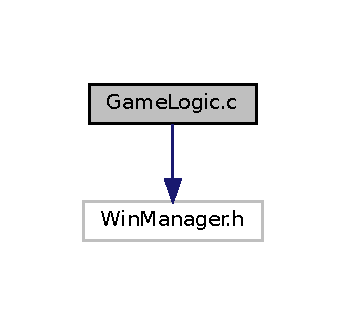
\includegraphics[width=166pt]{GameLogic_8c__incl}
\end{center}
\end{figure}
\subsection*{Functions}
\begin{DoxyCompactItemize}
\item 
void \mbox{\hyperlink{GameLogic_8c_a285c3f70c3743d8c4d1d64574cbaeccf}{start\+New\+Game}} ()
\begin{DoxyCompactList}\small\item\em Função\+: Inicia e determina o que acontece no jogo. \end{DoxyCompactList}\item 
void \mbox{\hyperlink{GameLogic_8c_a7cce67ceb88c653b0572dbb89add5d38}{player\+Checkers}} ()
\begin{DoxyCompactList}\small\item\em Função\+: Verificar Status das Estruturas e tropas do Player. \end{DoxyCompactList}\item 
void \mbox{\hyperlink{GameLogic_8c_a3745a14194c42945ac994ba20448e370}{on\+Game\+Routine}} ()
\begin{DoxyCompactList}\small\item\em Função\+: Chama as Funções Para Atualizar o Jogo. \end{DoxyCompactList}\item 
void \mbox{\hyperlink{GameLogic_8c_acfc6eb449ca115b62b027250c46597b3}{enemy\+Checkers}} ()
\begin{DoxyCompactList}\small\item\em Função\+: Verificar Status dos Prédios e Tropas do PC. \end{DoxyCompactList}\item 
void \mbox{\hyperlink{GameLogic_8c_ad3f949a3837869c04ca3115c5c1558b1}{game\+Checkers}} ()
\begin{DoxyCompactList}\small\item\em Função\+: Atualizar Status Gerais. \end{DoxyCompactList}\item 
void \mbox{\hyperlink{GameLogic_8c_aa47d7322cce56921933f620dde8dc20b}{player\+Controllers}} ()
\begin{DoxyCompactList}\small\item\em Função\+: Verificar Criação de Recursos e Tropas do Player. \end{DoxyCompactList}\item 
void \mbox{\hyperlink{GameLogic_8c_ace3531b6b91cdfc6e5efb802e79079c5}{enemy\+Controllers}} ()
\begin{DoxyCompactList}\small\item\em Função\+: Verificar Criação de Recursos e Tropas do PC. \end{DoxyCompactList}\item 
void \mbox{\hyperlink{GameLogic_8c_a9eb420ce9f7c7664de188d277f069309}{game\+Controllers}} ()
\begin{DoxyCompactList}\small\item\em Função\+: Atualizar Recursos e Tropas Gerais. \end{DoxyCompactList}\item 
void \mbox{\hyperlink{GameLogic_8c_aa8ec071ce9e46c870e5eef1443f78969}{refresh\+Game}} ()
\begin{DoxyCompactList}\small\item\em Função\+: Atualizar a Tela. \end{DoxyCompactList}\item 
void \mbox{\hyperlink{GameLogic_8c_ac5d72dfe00aec01540c4ffbf3c17168e}{pause\+Game\+Routine}} ()
\begin{DoxyCompactList}\small\item\em Função\+: Controlar as Opções no Menu de Pause. \end{DoxyCompactList}\item 
void \mbox{\hyperlink{GameLogic_8c_a588696d89f65cab797ac3aa09db8ace5}{print\+Game}} ()
\begin{DoxyCompactList}\small\item\em Função\+: Printar na Tela o Jogo. \end{DoxyCompactList}\item 
void \mbox{\hyperlink{GameLogic_8c_a9255c729e3e0425e5f6f420ef18d19bd}{alloc\+Game}} ()
\begin{DoxyCompactList}\small\item\em Função\+: Iniciar e Alocar Pré-\/\+Requisitos para o Jogo. \end{DoxyCompactList}\item 
void \mbox{\hyperlink{GameLogic_8c_ab7c9ee132f977dd2efd33ab66509d650}{destroy\+Game}} ()
\begin{DoxyCompactList}\small\item\em Função\+: Desaloca e Finaliza as Janelas. \end{DoxyCompactList}\item 
void \mbox{\hyperlink{GameLogic_8c_ac42f6d85eb40dfdfadbf9933d885b4c1}{save\+Game}} ()
\begin{DoxyCompactList}\small\item\em Função\+: Salvar o Jogo. \end{DoxyCompactList}\item 
int \mbox{\hyperlink{GameLogic_8c_ac340004cff52617fb540899b03191a9b}{load\+Game}} ()
\begin{DoxyCompactList}\small\item\em Função\+: Carregar um Jogo Salvo. \end{DoxyCompactList}\end{DoxyCompactItemize}
\subsection*{Variables}
\begin{DoxyCompactItemize}
\item 
W\+I\+N\+D\+OW $\ast$ \mbox{\hyperlink{GameLogic_8c_aa578a767fc3d38ab4b0211e552ed41cd}{game\+Win}}
\item 
W\+I\+N\+D\+OW $\ast$ \mbox{\hyperlink{GameLogic_8c_a81cc11227a869b90adbf28221ec125a7}{status\+Win}}
\item 
int \mbox{\hyperlink{GameLogic_8c_ab7ad0796d84021de0fd46246b3d5096f}{game\+State}}
\end{DoxyCompactItemize}


\subsection{Function Documentation}
\mbox{\Hypertarget{GameLogic_8c_a9255c729e3e0425e5f6f420ef18d19bd}\label{GameLogic_8c_a9255c729e3e0425e5f6f420ef18d19bd}} 
\index{Game\+Logic.\+c@{Game\+Logic.\+c}!alloc\+Game@{alloc\+Game}}
\index{alloc\+Game@{alloc\+Game}!Game\+Logic.\+c@{Game\+Logic.\+c}}
\subsubsection{\texorpdfstring{alloc\+Game()}{allocGame()}}
{\footnotesize\ttfamily void alloc\+Game (\begin{DoxyParamCaption}{ }\end{DoxyParamCaption})}



Função\+: Iniciar e Alocar Pré-\/\+Requisitos para o Jogo. 

Descrição\+: A Função aloca e cria as janelas do jogo e do status, aloca o mapa do jogo e o inicializa.

Parâmetros\+: 
\begin{DoxyParams}{Parameters}
{\em sem} & parâmetros\\
\hline
\end{DoxyParams}
Valor retornado\+: \begin{DoxyReturn}{Returns}
função void -\/ A função não retorna nada
\end{DoxyReturn}
Assertiva de entrada\+: Sem parâmetros

Assertiva de saída\+: Função void \mbox{\Hypertarget{GameLogic_8c_ab7c9ee132f977dd2efd33ab66509d650}\label{GameLogic_8c_ab7c9ee132f977dd2efd33ab66509d650}} 
\index{Game\+Logic.\+c@{Game\+Logic.\+c}!destroy\+Game@{destroy\+Game}}
\index{destroy\+Game@{destroy\+Game}!Game\+Logic.\+c@{Game\+Logic.\+c}}
\subsubsection{\texorpdfstring{destroy\+Game()}{destroyGame()}}
{\footnotesize\ttfamily void destroy\+Game (\begin{DoxyParamCaption}{ }\end{DoxyParamCaption})}



Função\+: Desaloca e Finaliza as Janelas. 

Descrição\+: A Função desaloca a janela utilizada para o jogo e para o status e desaloca o mapa do jogo. Então limpa o terminal e atualiza a tela.

Parâmetros\+: 
\begin{DoxyParams}{Parameters}
{\em sem} & parâmetros\\
\hline
\end{DoxyParams}
Valor retornado\+: \begin{DoxyReturn}{Returns}
função void -\/ A função não retorna nada
\end{DoxyReturn}
Assertiva de entrada\+: Sem parâmetros

Assertiva de saída\+: Função void \mbox{\Hypertarget{GameLogic_8c_acfc6eb449ca115b62b027250c46597b3}\label{GameLogic_8c_acfc6eb449ca115b62b027250c46597b3}} 
\index{Game\+Logic.\+c@{Game\+Logic.\+c}!enemy\+Checkers@{enemy\+Checkers}}
\index{enemy\+Checkers@{enemy\+Checkers}!Game\+Logic.\+c@{Game\+Logic.\+c}}
\subsubsection{\texorpdfstring{enemy\+Checkers()}{enemyCheckers()}}
{\footnotesize\ttfamily void enemy\+Checkers (\begin{DoxyParamCaption}{ }\end{DoxyParamCaption})}



Função\+: Verificar Status dos Prédios e Tropas do PC. 

Descrição\+: A Função chama funções para verificar a vida dos prédios e a quantidade de tropas do PC.

Parâmetros\+: 
\begin{DoxyParams}{Parameters}
{\em sem} & parâmetros\\
\hline
\end{DoxyParams}
Valor retornado\+: \begin{DoxyReturn}{Returns}
função void -\/ A função não retorna nada
\end{DoxyReturn}
Assertiva de entrada\+: Sem parâmetros

Assertiva de saída\+: Função void \mbox{\Hypertarget{GameLogic_8c_ace3531b6b91cdfc6e5efb802e79079c5}\label{GameLogic_8c_ace3531b6b91cdfc6e5efb802e79079c5}} 
\index{Game\+Logic.\+c@{Game\+Logic.\+c}!enemy\+Controllers@{enemy\+Controllers}}
\index{enemy\+Controllers@{enemy\+Controllers}!Game\+Logic.\+c@{Game\+Logic.\+c}}
\subsubsection{\texorpdfstring{enemy\+Controllers()}{enemyControllers()}}
{\footnotesize\ttfamily void enemy\+Controllers (\begin{DoxyParamCaption}{ }\end{DoxyParamCaption})}



Função\+: Verificar Criação de Recursos e Tropas do PC. 

Descrição\+: A Função chama funções para verificar a mineração de recursos e a criação de tropas do PC.

Parâmetros\+: 
\begin{DoxyParams}{Parameters}
{\em sem} & parâmetros\\
\hline
\end{DoxyParams}
Valor retornado\+: \begin{DoxyReturn}{Returns}
função void -\/ A função não retorna nada
\end{DoxyReturn}
Assertiva de entrada\+: Sem parâmetros

Assertiva de saída\+: Função void \mbox{\Hypertarget{GameLogic_8c_ad3f949a3837869c04ca3115c5c1558b1}\label{GameLogic_8c_ad3f949a3837869c04ca3115c5c1558b1}} 
\index{Game\+Logic.\+c@{Game\+Logic.\+c}!game\+Checkers@{game\+Checkers}}
\index{game\+Checkers@{game\+Checkers}!Game\+Logic.\+c@{Game\+Logic.\+c}}
\subsubsection{\texorpdfstring{game\+Checkers()}{gameCheckers()}}
{\footnotesize\ttfamily void game\+Checkers (\begin{DoxyParamCaption}{ }\end{DoxyParamCaption})}



Função\+: Atualizar Status Gerais. 

Descrição\+: A Função chama funções de checagem de mudança de status em tropas e prédios do player e do PC.

Parâmetros\+: 
\begin{DoxyParams}{Parameters}
{\em sem} & parâmetros\\
\hline
\end{DoxyParams}
Valor retornado\+: \begin{DoxyReturn}{Returns}
função void -\/ A função não retorna nada
\end{DoxyReturn}
Assertiva de entrada\+: Sem parâmetros

Assertiva de saída\+: Função void \mbox{\Hypertarget{GameLogic_8c_a9eb420ce9f7c7664de188d277f069309}\label{GameLogic_8c_a9eb420ce9f7c7664de188d277f069309}} 
\index{Game\+Logic.\+c@{Game\+Logic.\+c}!game\+Controllers@{game\+Controllers}}
\index{game\+Controllers@{game\+Controllers}!Game\+Logic.\+c@{Game\+Logic.\+c}}
\subsubsection{\texorpdfstring{game\+Controllers()}{gameControllers()}}
{\footnotesize\ttfamily void game\+Controllers (\begin{DoxyParamCaption}{ }\end{DoxyParamCaption})}



Função\+: Atualizar Recursos e Tropas Gerais. 

Descrição\+: A Função chama funções de verificação da mineração de recursos e da criação de tropas.

Parâmetros\+: 
\begin{DoxyParams}{Parameters}
{\em sem} & parâmetros\\
\hline
\end{DoxyParams}
Valor retornado\+: \begin{DoxyReturn}{Returns}
função void -\/ A função não retorna nada
\end{DoxyReturn}
Assertiva de entrada\+: Sem parâmetros

Assertiva de saída\+: Função void \mbox{\Hypertarget{GameLogic_8c_ac340004cff52617fb540899b03191a9b}\label{GameLogic_8c_ac340004cff52617fb540899b03191a9b}} 
\index{Game\+Logic.\+c@{Game\+Logic.\+c}!load\+Game@{load\+Game}}
\index{load\+Game@{load\+Game}!Game\+Logic.\+c@{Game\+Logic.\+c}}
\subsubsection{\texorpdfstring{load\+Game()}{loadGame()}}
{\footnotesize\ttfamily int load\+Game (\begin{DoxyParamCaption}{ }\end{DoxyParamCaption})}



Função\+: Carregar um Jogo Salvo. 

Descrição\+: A Função abre o arquivo de save e lê todos os dados da base, prédios e tropas do player e do PC. Caso não exista um save, é mostrado uma mensagem na tela.

Parâmetros\+: 
\begin{DoxyParams}{Parameters}
{\em sem} & parâmetros\\
\hline
\end{DoxyParams}
Valor retornado\+: \begin{DoxyReturn}{Returns}
0 -\/ se não existir um arquivo de save válido 

1 -\/ se o load ocorrer sem problemas
\end{DoxyReturn}
Assertiva de entrada\+: Sem parâmetros

Assertiva de saída\+: A função retorna valores fixos. \mbox{\Hypertarget{GameLogic_8c_a3745a14194c42945ac994ba20448e370}\label{GameLogic_8c_a3745a14194c42945ac994ba20448e370}} 
\index{Game\+Logic.\+c@{Game\+Logic.\+c}!on\+Game\+Routine@{on\+Game\+Routine}}
\index{on\+Game\+Routine@{on\+Game\+Routine}!Game\+Logic.\+c@{Game\+Logic.\+c}}
\subsubsection{\texorpdfstring{on\+Game\+Routine()}{onGameRoutine()}}
{\footnotesize\ttfamily void on\+Game\+Routine (\begin{DoxyParamCaption}{ }\end{DoxyParamCaption})}



Função\+: Chama as Funções Para Atualizar o Jogo. 

Descrição\+: A Função chama funções de atualizar a tela, mover tropas, verificar recursos e tropas. Ou seja, atualiza tudo dentro do jogo.

Parâmetros\+: 
\begin{DoxyParams}{Parameters}
{\em sem} & parâmetros\\
\hline
\end{DoxyParams}
Valor retornado\+: \begin{DoxyReturn}{Returns}
função void -\/ A função não retorna nada
\end{DoxyReturn}
Assertiva de entrada\+: Sem parâmetros

Assertiva de saída\+: Função void \mbox{\Hypertarget{GameLogic_8c_ac5d72dfe00aec01540c4ffbf3c17168e}\label{GameLogic_8c_ac5d72dfe00aec01540c4ffbf3c17168e}} 
\index{Game\+Logic.\+c@{Game\+Logic.\+c}!pause\+Game\+Routine@{pause\+Game\+Routine}}
\index{pause\+Game\+Routine@{pause\+Game\+Routine}!Game\+Logic.\+c@{Game\+Logic.\+c}}
\subsubsection{\texorpdfstring{pause\+Game\+Routine()}{pauseGameRoutine()}}
{\footnotesize\ttfamily void pause\+Game\+Routine (\begin{DoxyParamCaption}{ }\end{DoxyParamCaption})}



Função\+: Controlar as Opções no Menu de Pause. 

Descrição\+: A Função volta ao jogo, salva o jogo ou saí do jogo de acordo com a opção selecionada no menu de Pause.

Parâmetros\+: 
\begin{DoxyParams}{Parameters}
{\em sem} & parâmetros\\
\hline
\end{DoxyParams}
Valor retornado\+: \begin{DoxyReturn}{Returns}
função void -\/ A função não retorna nada
\end{DoxyReturn}
Assertiva de entrada\+: Sem parâmetros

Assertiva de saída\+: Função void \mbox{\Hypertarget{GameLogic_8c_a7cce67ceb88c653b0572dbb89add5d38}\label{GameLogic_8c_a7cce67ceb88c653b0572dbb89add5d38}} 
\index{Game\+Logic.\+c@{Game\+Logic.\+c}!player\+Checkers@{player\+Checkers}}
\index{player\+Checkers@{player\+Checkers}!Game\+Logic.\+c@{Game\+Logic.\+c}}
\subsubsection{\texorpdfstring{player\+Checkers()}{playerCheckers()}}
{\footnotesize\ttfamily void player\+Checkers (\begin{DoxyParamCaption}{ }\end{DoxyParamCaption})}



Função\+: Verificar Status das Estruturas e tropas do Player. 

Descrição\+: A Função chama as funções para verificar se há batalhas entre tropas, se alguma tropa está atacando algum prédio ou base inimiga, qual a vida dos prédios do player e a quantidade de tropas que o player possui.

Parâmetros\+: 
\begin{DoxyParams}{Parameters}
{\em sem} & parâmetros\\
\hline
\end{DoxyParams}
Valor retornado\+: \begin{DoxyReturn}{Returns}
função void -\/ A função não retorna nada
\end{DoxyReturn}
Assertiva de entrada\+: Sem parâmetros

Assertiva de saída\+: Função void \mbox{\Hypertarget{GameLogic_8c_aa47d7322cce56921933f620dde8dc20b}\label{GameLogic_8c_aa47d7322cce56921933f620dde8dc20b}} 
\index{Game\+Logic.\+c@{Game\+Logic.\+c}!player\+Controllers@{player\+Controllers}}
\index{player\+Controllers@{player\+Controllers}!Game\+Logic.\+c@{Game\+Logic.\+c}}
\subsubsection{\texorpdfstring{player\+Controllers()}{playerControllers()}}
{\footnotesize\ttfamily void player\+Controllers (\begin{DoxyParamCaption}{ }\end{DoxyParamCaption})}



Função\+: Verificar Criação de Recursos e Tropas do Player. 

Descrição\+: A Função chama funções para verificar a mineração de recursos e a criação de tropas do player.

Parâmetros\+: 
\begin{DoxyParams}{Parameters}
{\em sem} & parâmetros\\
\hline
\end{DoxyParams}
Valor retornado\+: \begin{DoxyReturn}{Returns}
função void -\/ A função não retorna nada
\end{DoxyReturn}
Assertiva de entrada\+: Sem parâmetros

Assertiva de saída\+: Função void \mbox{\Hypertarget{GameLogic_8c_a588696d89f65cab797ac3aa09db8ace5}\label{GameLogic_8c_a588696d89f65cab797ac3aa09db8ace5}} 
\index{Game\+Logic.\+c@{Game\+Logic.\+c}!print\+Game@{print\+Game}}
\index{print\+Game@{print\+Game}!Game\+Logic.\+c@{Game\+Logic.\+c}}
\subsubsection{\texorpdfstring{print\+Game()}{printGame()}}
{\footnotesize\ttfamily void print\+Game (\begin{DoxyParamCaption}{ }\end{DoxyParamCaption})}



Função\+: Printar na Tela o Jogo. 

Descrição\+: A Função imprime os status do player, do PC e o mapa do jogo.

Parâmetros\+: 
\begin{DoxyParams}{Parameters}
{\em sem} & parâmetros\\
\hline
\end{DoxyParams}
Valor retornado\+: \begin{DoxyReturn}{Returns}
função void -\/ A função não retorna nada
\end{DoxyReturn}
Assertiva de entrada\+: Sem parâmetros

Assertiva de saída\+: Função void \mbox{\Hypertarget{GameLogic_8c_aa8ec071ce9e46c870e5eef1443f78969}\label{GameLogic_8c_aa8ec071ce9e46c870e5eef1443f78969}} 
\index{Game\+Logic.\+c@{Game\+Logic.\+c}!refresh\+Game@{refresh\+Game}}
\index{refresh\+Game@{refresh\+Game}!Game\+Logic.\+c@{Game\+Logic.\+c}}
\subsubsection{\texorpdfstring{refresh\+Game()}{refreshGame()}}
{\footnotesize\ttfamily void refresh\+Game (\begin{DoxyParamCaption}{ }\end{DoxyParamCaption})}



Função\+: Atualizar a Tela. 

Descrição\+: A Função atualiza a tela do jogo e dá um refresh.

Parâmetros\+: 
\begin{DoxyParams}{Parameters}
{\em sem} & parâmetros\\
\hline
\end{DoxyParams}
Valor retornado\+: \begin{DoxyReturn}{Returns}
função void -\/ A função apenas imprime o jogo na tela
\end{DoxyReturn}
Assertiva de entrada\+: Sem parâmetros

Assertiva de saída\+: Função void \mbox{\Hypertarget{GameLogic_8c_ac42f6d85eb40dfdfadbf9933d885b4c1}\label{GameLogic_8c_ac42f6d85eb40dfdfadbf9933d885b4c1}} 
\index{Game\+Logic.\+c@{Game\+Logic.\+c}!save\+Game@{save\+Game}}
\index{save\+Game@{save\+Game}!Game\+Logic.\+c@{Game\+Logic.\+c}}
\subsubsection{\texorpdfstring{save\+Game()}{saveGame()}}
{\footnotesize\ttfamily void save\+Game (\begin{DoxyParamCaption}{ }\end{DoxyParamCaption})}



Função\+: Salvar o Jogo. 

Descrição\+: A Função cria um arquivo binário e salva todos os dados da base, dos prédios e das tropas do player e do PC nele.

Parâmetros\+: 
\begin{DoxyParams}{Parameters}
{\em sem} & parâmetros\\
\hline
\end{DoxyParams}
Valor retornado\+: \begin{DoxyReturn}{Returns}
função void -\/ A função não retorna nada
\end{DoxyReturn}
Assertiva de entrada\+: Sem parâmetros

Assertiva de saída\+: Função void \mbox{\Hypertarget{GameLogic_8c_a285c3f70c3743d8c4d1d64574cbaeccf}\label{GameLogic_8c_a285c3f70c3743d8c4d1d64574cbaeccf}} 
\index{Game\+Logic.\+c@{Game\+Logic.\+c}!start\+New\+Game@{start\+New\+Game}}
\index{start\+New\+Game@{start\+New\+Game}!Game\+Logic.\+c@{Game\+Logic.\+c}}
\subsubsection{\texorpdfstring{start\+New\+Game()}{startNewGame()}}
{\footnotesize\ttfamily void start\+New\+Game (\begin{DoxyParamCaption}{ }\end{DoxyParamCaption})}



Função\+: Inicia e determina o que acontece no jogo. 

Descrição\+: A Função é responsável por alocar tudo que o jogo vai usar, atualizar a tela, verificar se o jogo está em Play ou em Pause. É onde o loop do jogo acontece. Quando a vida da base de um dos jogadores se torna 0, a função encerra o jogo e finaliza tudo.

Parâmetros\+: 
\begin{DoxyParams}{Parameters}
{\em sem} & parâmetros\\
\hline
\end{DoxyParams}
Valor retornado\+: \begin{DoxyReturn}{Returns}
função void -\/ a função não retorna nada
\end{DoxyReturn}
Assertiva de entrada\+: Sem parâmetros

Assertiva de saída\+: Função void 

\subsection{Variable Documentation}
\mbox{\Hypertarget{GameLogic_8c_ab7ad0796d84021de0fd46246b3d5096f}\label{GameLogic_8c_ab7ad0796d84021de0fd46246b3d5096f}} 
\index{Game\+Logic.\+c@{Game\+Logic.\+c}!game\+State@{game\+State}}
\index{game\+State@{game\+State}!Game\+Logic.\+c@{Game\+Logic.\+c}}
\subsubsection{\texorpdfstring{game\+State}{gameState}}
{\footnotesize\ttfamily int game\+State}

Flag para identificar se o jogo está pausado ou rodando \mbox{\Hypertarget{GameLogic_8c_aa578a767fc3d38ab4b0211e552ed41cd}\label{GameLogic_8c_aa578a767fc3d38ab4b0211e552ed41cd}} 
\index{Game\+Logic.\+c@{Game\+Logic.\+c}!game\+Win@{game\+Win}}
\index{game\+Win@{game\+Win}!Game\+Logic.\+c@{Game\+Logic.\+c}}
\subsubsection{\texorpdfstring{game\+Win}{gameWin}}
{\footnotesize\ttfamily W\+I\+N\+D\+OW$\ast$ game\+Win}

Janela do jogo \mbox{\Hypertarget{GameLogic_8c_a81cc11227a869b90adbf28221ec125a7}\label{GameLogic_8c_a81cc11227a869b90adbf28221ec125a7}} 
\index{Game\+Logic.\+c@{Game\+Logic.\+c}!status\+Win@{status\+Win}}
\index{status\+Win@{status\+Win}!Game\+Logic.\+c@{Game\+Logic.\+c}}
\subsubsection{\texorpdfstring{status\+Win}{statusWin}}
{\footnotesize\ttfamily W\+I\+N\+D\+OW$\ast$ status\+Win}

Janela dos status 
\hypertarget{main_8c}{}\section{main.\+c File Reference}
\label{main_8c}\index{main.\+c@{main.\+c}}
{\ttfamily \#include \char`\"{}Win\+Manager.\+h\char`\"{}}\newline
Include dependency graph for main.\+c\+:
\nopagebreak
\begin{figure}[H]
\begin{center}
\leavevmode
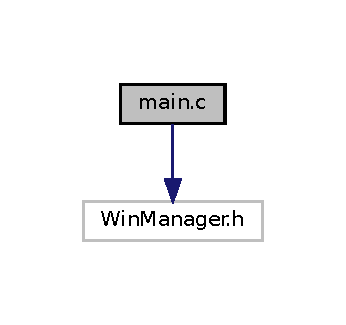
\includegraphics[width=166pt]{main_8c__incl}
\end{center}
\end{figure}
\subsection*{Functions}
\begin{DoxyCompactItemize}
\item 
int \mbox{\hyperlink{main_8c_ae66f6b31b5ad750f1fe042a706a4e3d4}{main}} ()
\end{DoxyCompactItemize}


\subsection{Function Documentation}
\mbox{\Hypertarget{main_8c_ae66f6b31b5ad750f1fe042a706a4e3d4}\label{main_8c_ae66f6b31b5ad750f1fe042a706a4e3d4}} 
\index{main.\+c@{main.\+c}!main@{main}}
\index{main@{main}!main.\+c@{main.\+c}}
\subsubsection{\texorpdfstring{main()}{main()}}
{\footnotesize\ttfamily int main (\begin{DoxyParamCaption}{ }\end{DoxyParamCaption})}

main 
\hypertarget{MapFunc_8c}{}\section{Map\+Func.\+c File Reference}
\label{MapFunc_8c}\index{Map\+Func.\+c@{Map\+Func.\+c}}
{\ttfamily \#include \char`\"{}Map\+Func.\+h\char`\"{}}\newline
Include dependency graph for Map\+Func.\+c\+:
\nopagebreak
\begin{figure}[H]
\begin{center}
\leavevmode
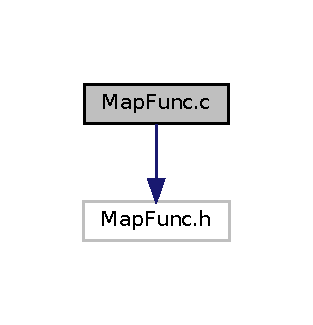
\includegraphics[width=150pt]{MapFunc_8c__incl}
\end{center}
\end{figure}
\subsection*{Functions}
\begin{DoxyCompactItemize}
\item 
char $\ast$$\ast$ \mbox{\hyperlink{MapFunc_8c_ad96ef7faf3539ffcf3771457543ba70c}{alloc\+Map}} (char $\ast$$\ast$map, int y, int x)
\begin{DoxyCompactList}\small\item\em Função\+: Alocar o Mapa do Jogo. \end{DoxyCompactList}\item 
char $\ast$$\ast$ \mbox{\hyperlink{MapFunc_8c_a94d35ed1335c3aac5b645acb3fa56506}{dealloc\+Map}} (char $\ast$$\ast$map)
\begin{DoxyCompactList}\small\item\em Função\+: Desalocar o Mapa do Jogo. \end{DoxyCompactList}\item 
void \mbox{\hyperlink{MapFunc_8c_a5fc3e5c84a92b563265072f42dc861e8}{set\+Base\+On\+Map}} (char $\ast$$\ast$map, Base $\ast$bc, int x, int y, int width, int height, int who, int save)
\begin{DoxyCompactList}\small\item\em Função\+: Colocar no Mapa a Base. \end{DoxyCompactList}\item 
void \mbox{\hyperlink{MapFunc_8c_aab712fd52de5ba0d8d02ad69e9fe2c62}{set\+Build\+On\+Map}} (char $\ast$$\ast$map, Build $\ast$b, int x, int y, int width, int height, int type, int who, int save)
\begin{DoxyCompactList}\small\item\em Função\+: Colocar no Mapa um prédio. \end{DoxyCompactList}\item 
void \mbox{\hyperlink{MapFunc_8c_a736892c9b435fd3b70467beadb7a3d22}{set\+Troop\+On\+Map}} (char $\ast$$\ast$map, Troop $\ast$t, int x, int y, int type, int who, int save)
\begin{DoxyCompactList}\small\item\em Função\+: Colocar no Mapa a Tropa. \end{DoxyCompactList}\item 
void \mbox{\hyperlink{MapFunc_8c_a0e1cb1f76b3781662505eccdbe1a40d3}{set\+Map}} (char $\ast$$\ast$map, int save)
\begin{DoxyCompactList}\small\item\em Função\+: Setar a Matriz do Mapa. \end{DoxyCompactList}\item 
void \mbox{\hyperlink{MapFunc_8c_aa3e05dc8fbb4d9c39fe64dc3241d8e10}{print\+Map}} (W\+I\+N\+D\+OW $\ast$win, char $\ast$$\ast$map)
\begin{DoxyCompactList}\small\item\em Função\+: Imprimir o Mapa na Window. \end{DoxyCompactList}\end{DoxyCompactItemize}
\subsection*{Variables}
\begin{DoxyCompactItemize}
\item 
int \mbox{\hyperlink{MapFunc_8c_a166056ba9deace5bfd048d049a4d282a}{map\+\_\+y}}
\item 
int \mbox{\hyperlink{MapFunc_8c_aa7def7b32d142160e043b9b8926b6c5d}{map\+\_\+x}}
\end{DoxyCompactItemize}


\subsection{Function Documentation}
\mbox{\Hypertarget{MapFunc_8c_ad96ef7faf3539ffcf3771457543ba70c}\label{MapFunc_8c_ad96ef7faf3539ffcf3771457543ba70c}} 
\index{Map\+Func.\+c@{Map\+Func.\+c}!alloc\+Map@{alloc\+Map}}
\index{alloc\+Map@{alloc\+Map}!Map\+Func.\+c@{Map\+Func.\+c}}
\subsubsection{\texorpdfstring{alloc\+Map()}{allocMap()}}
{\footnotesize\ttfamily char$\ast$$\ast$ alloc\+Map (\begin{DoxyParamCaption}\item[{char $\ast$$\ast$}]{map,  }\item[{int}]{y,  }\item[{int}]{x }\end{DoxyParamCaption})}



Função\+: Alocar o Mapa do Jogo. 

Descrição\+: A Função recebe uma matriz do tipo char, e o numero de linhas e de colunas que essa matriz (mapa do jogo) vai possuir. A matriz é alocada e retornada.

Parâmetros\+: 
\begin{DoxyParams}{Parameters}
{\em char$\ast$$\ast$} & map -\/ matriz do tipo char que vai ser alocada \\
\hline
{\em int} & x -\/ número de linhas da matriz \\
\hline
{\em int} & y -\/ número de colunas da matriz\\
\hline
\end{DoxyParams}
Valor retornado\+: \begin{DoxyReturn}{Returns}
char$\ast$$\ast$ map -\/ matriz alocada
\end{DoxyReturn}
Assertiva de entrada\+: char$\ast$$\ast$ map == N\+U\+LL int x $>$ 0 int y $>$ 0

Assertiva de saída\+: char$\ast$$\ast$ map != N\+U\+LL \mbox{\Hypertarget{MapFunc_8c_a94d35ed1335c3aac5b645acb3fa56506}\label{MapFunc_8c_a94d35ed1335c3aac5b645acb3fa56506}} 
\index{Map\+Func.\+c@{Map\+Func.\+c}!dealloc\+Map@{dealloc\+Map}}
\index{dealloc\+Map@{dealloc\+Map}!Map\+Func.\+c@{Map\+Func.\+c}}
\subsubsection{\texorpdfstring{dealloc\+Map()}{deallocMap()}}
{\footnotesize\ttfamily char$\ast$$\ast$ dealloc\+Map (\begin{DoxyParamCaption}\item[{char $\ast$$\ast$}]{map }\end{DoxyParamCaption})}



Função\+: Desalocar o Mapa do Jogo. 

Descrição\+: A Função recebe uma matriz (mapa do jogo) do tipo char e a desaloca. Então retorna a matriz desalocada.

Parâmetros\+: 
\begin{DoxyParams}{Parameters}
{\em char$\ast$$\ast$} & map -\/ matriz do tipo char que vai ser desalocada\\
\hline
\end{DoxyParams}
Valor retornado\+: \begin{DoxyReturn}{Returns}
char$\ast$$\ast$ map -\/ matriz desalocada
\end{DoxyReturn}
Assertiva de entrada\+: char$\ast$$\ast$ map == N\+U\+LL

Assertiva de saída\+: char$\ast$$\ast$ map == N\+U\+LL \mbox{\Hypertarget{MapFunc_8c_aa3e05dc8fbb4d9c39fe64dc3241d8e10}\label{MapFunc_8c_aa3e05dc8fbb4d9c39fe64dc3241d8e10}} 
\index{Map\+Func.\+c@{Map\+Func.\+c}!print\+Map@{print\+Map}}
\index{print\+Map@{print\+Map}!Map\+Func.\+c@{Map\+Func.\+c}}
\subsubsection{\texorpdfstring{print\+Map()}{printMap()}}
{\footnotesize\ttfamily void print\+Map (\begin{DoxyParamCaption}\item[{W\+I\+N\+D\+OW $\ast$}]{win,  }\item[{char $\ast$$\ast$}]{map }\end{DoxyParamCaption})}



Função\+: Imprimir o Mapa na Window. 

Descrição\+: A Função recebe uma matriz (mapa do jogo) do tipo char e uma janela (ncurses). Então ela printa na tela o mapa, com as bases, prédios e tropas. Ela também é responsável pelas cores printadas.

Parâmetros\+: 
\begin{DoxyParams}{Parameters}
{\em char$\ast$$\ast$} & map -\/ matriz (mapa) do tipo char \\
\hline
{\em W\+I\+N\+D\+O\+W$\ast$} & win -\/ uma janela\\
\hline
\end{DoxyParams}
Valor retornado\+: \begin{DoxyReturn}{Returns}
função void. É uma função de atualização de tela
\end{DoxyReturn}
Assertiva de entrada\+: char$\ast$$\ast$ map != N\+U\+LL

Assertiva de saída\+: Função void \mbox{\Hypertarget{MapFunc_8c_a5fc3e5c84a92b563265072f42dc861e8}\label{MapFunc_8c_a5fc3e5c84a92b563265072f42dc861e8}} 
\index{Map\+Func.\+c@{Map\+Func.\+c}!set\+Base\+On\+Map@{set\+Base\+On\+Map}}
\index{set\+Base\+On\+Map@{set\+Base\+On\+Map}!Map\+Func.\+c@{Map\+Func.\+c}}
\subsubsection{\texorpdfstring{set\+Base\+On\+Map()}{setBaseOnMap()}}
{\footnotesize\ttfamily void set\+Base\+On\+Map (\begin{DoxyParamCaption}\item[{char $\ast$$\ast$}]{map,  }\item[{Base $\ast$}]{bc,  }\item[{int}]{x,  }\item[{int}]{y,  }\item[{int}]{width,  }\item[{int}]{height,  }\item[{int}]{who,  }\item[{int}]{save }\end{DoxyParamCaption})}



Função\+: Colocar no Mapa a Base. 

Descrição\+: A Função recebe uma matriz (mapa do jogo) do tipo char, uma struct de uma base, a posição que essa base vai ficar, a altura e a largura dessa base, uma flag para identificar se a base é do player ou do PC e uma flag para identificar se a base é de um jogo novo ou de um save. A base é setada e escrita no mapa como \textquotesingle{}B\textquotesingle{} ou \textquotesingle{}C\textquotesingle{}, dependendo da flag, na posição que foi mandada.

Parâmetros\+: 
\begin{DoxyParams}{Parameters}
{\em char$\ast$$\ast$} & map -\/ matriz (mapa) do tipo char \\
\hline
{\em Base$\ast$} & bc -\/ uma struct para a base \\
\hline
{\em int} & x -\/ coordenada x da base \\
\hline
{\em int} & y -\/ coordenada y da base \\
\hline
{\em int} & width -\/ largura da base \\
\hline
{\em int} & height -\/ altura da base \\
\hline
{\em int} & who -\/ flag para identificar se a base é do Player (0) ou do PC (1) \\
\hline
{\em int} & save -\/ flag para identificar se a base está sendo carregada de um jogo novo (0) ou de um save (1)\\
\hline
\end{DoxyParams}
Valor retornado\+: \begin{DoxyReturn}{Returns}
função void. Os valores são mudados por referência
\end{DoxyReturn}
Assertiva de entrada\+: char$\ast$$\ast$ map != N\+U\+LL Base$\ast$ bc != N\+U\+LL int x $>$= 0 int y $>$= 0 int width $>$ 0 int height $>$ 0 int who == 0 $\vert$$\vert$ who == 1 int save == 0 $\vert$$\vert$ save == 1

Assertiva de saída\+: Função void \mbox{\Hypertarget{MapFunc_8c_aab712fd52de5ba0d8d02ad69e9fe2c62}\label{MapFunc_8c_aab712fd52de5ba0d8d02ad69e9fe2c62}} 
\index{Map\+Func.\+c@{Map\+Func.\+c}!set\+Build\+On\+Map@{set\+Build\+On\+Map}}
\index{set\+Build\+On\+Map@{set\+Build\+On\+Map}!Map\+Func.\+c@{Map\+Func.\+c}}
\subsubsection{\texorpdfstring{set\+Build\+On\+Map()}{setBuildOnMap()}}
{\footnotesize\ttfamily void set\+Build\+On\+Map (\begin{DoxyParamCaption}\item[{char $\ast$$\ast$}]{map,  }\item[{Build $\ast$}]{b,  }\item[{int}]{x,  }\item[{int}]{y,  }\item[{int}]{width,  }\item[{int}]{height,  }\item[{int}]{type,  }\item[{int}]{who,  }\item[{int}]{save }\end{DoxyParamCaption})}



Função\+: Colocar no Mapa um prédio. 

Descrição\+: A Função recebe uma matriz (mapa do jogo) do tipo char, uma struct de uma prédio, a posição que esse prédio vai ficar, a altura e a largura desse prédio, uma flag para identificar qual o tipo desse prédio, uma flag para identificar se o prédio é do player ou do PC e uma flag para identificar se o prédio é de um jogo novo ou de um save. O prédio é setado e escrito no mapa na posição que foi mandado, que, dependendo das flags, fica como\+: \textquotesingle{}X\textquotesingle{} -\/ prédio de type 0 do player \textquotesingle{}Y\textquotesingle{} -\/ prédio do type 1 do player \textquotesingle{}Z\textquotesingle{} -\/ prédio do type 2 do player \textquotesingle{}L\textquotesingle{} -\/ prédio do type 0 do PC \textquotesingle{}M\textquotesingle{} -\/ prédio do type 1 do PC \textquotesingle{}N\textquotesingle{} -\/ prédio do type 2 do PC

Parâmetros\+: 
\begin{DoxyParams}{Parameters}
{\em char$\ast$$\ast$} & map -\/ matriz (mapa) do tipo char \\
\hline
{\em Build$\ast$} & b -\/ uma struct para o prédio \\
\hline
{\em int} & x -\/ coordenada x do prédio \\
\hline
{\em int} & y -\/ coordenada y do prédio \\
\hline
{\em int} & width -\/ largura do prédio \\
\hline
{\em int} & height -\/ altura do prédio \\
\hline
{\em int} & type -\/ flag para identificar o tipo do prédio \\
\hline
{\em int} & who -\/ flag para identificar se o prédio é do Player (0) ou do PC (1) \\
\hline
{\em int} & save -\/ flag para identificar se o prédio está sendo carregado de um jogo novo (0) ou de um save (1)\\
\hline
\end{DoxyParams}
Valor retornado\+: \begin{DoxyReturn}{Returns}
função void. Os valores são mudados por referência
\end{DoxyReturn}
Assertiva de entrada\+: char$\ast$$\ast$ map != N\+U\+LL Build$\ast$ b != N\+U\+LL int x $>$= 0 int y $>$= 0 int width $>$ 0 int height $>$ 0 int type == 0 $\vert$$\vert$ type == 1 $\vert$$\vert$ type == 2 int who == 0 $\vert$$\vert$ who == 1 int save == 0 $\vert$$\vert$ save == 1

Assertiva de saída\+: Função void \mbox{\Hypertarget{MapFunc_8c_a0e1cb1f76b3781662505eccdbe1a40d3}\label{MapFunc_8c_a0e1cb1f76b3781662505eccdbe1a40d3}} 
\index{Map\+Func.\+c@{Map\+Func.\+c}!set\+Map@{set\+Map}}
\index{set\+Map@{set\+Map}!Map\+Func.\+c@{Map\+Func.\+c}}
\subsubsection{\texorpdfstring{set\+Map()}{setMap()}}
{\footnotesize\ttfamily void set\+Map (\begin{DoxyParamCaption}\item[{char $\ast$$\ast$}]{map,  }\item[{int}]{save }\end{DoxyParamCaption})}



Função\+: Setar a Matriz do Mapa. 

Descrição\+: A Função recebe uma matriz (mapa do jogo) do tipo char e uma flag que identifica se o jogo é novo ou um save, então ela preenche o mapa com \textquotesingle{}.\textquotesingle{} .Depois é colocado as bases, prédios e tropas do player e do PC

Parâmetros\+: 
\begin{DoxyParams}{Parameters}
{\em char$\ast$$\ast$} & map -\/ matriz (mapa) do tipo char \\
\hline
{\em int} & save -\/ flag para identificar se o mapa vai ser setado para um jogo novo (0) ou para um save (1)\\
\hline
\end{DoxyParams}
Valor retornado\+: \begin{DoxyReturn}{Returns}
função void. Os valores são mudados por referência
\end{DoxyReturn}
Assertiva de entrada\+: char$\ast$$\ast$ map != N\+U\+LL int save == 0 $\vert$$\vert$ save == 1

Assertiva de saída\+: Função void \mbox{\Hypertarget{MapFunc_8c_a736892c9b435fd3b70467beadb7a3d22}\label{MapFunc_8c_a736892c9b435fd3b70467beadb7a3d22}} 
\index{Map\+Func.\+c@{Map\+Func.\+c}!set\+Troop\+On\+Map@{set\+Troop\+On\+Map}}
\index{set\+Troop\+On\+Map@{set\+Troop\+On\+Map}!Map\+Func.\+c@{Map\+Func.\+c}}
\subsubsection{\texorpdfstring{set\+Troop\+On\+Map()}{setTroopOnMap()}}
{\footnotesize\ttfamily void set\+Troop\+On\+Map (\begin{DoxyParamCaption}\item[{char $\ast$$\ast$}]{map,  }\item[{Troop $\ast$}]{t,  }\item[{int}]{x,  }\item[{int}]{y,  }\item[{int}]{type,  }\item[{int}]{who,  }\item[{int}]{save }\end{DoxyParamCaption})}



Função\+: Colocar no Mapa a Tropa. 

Descrição\+: A Função recebe uma matriz (mapa do jogo) do tipo char, uma struct de uma tropa, a posição que essa tropa vai ficar, uma flag para identificar qual o tipo de tropa, uma flag para identificar se a tropa é do player ou do PC e uma flag para identificar se a tropa é de um jogo novo ou de um save. A tropa é setada e escrita no mapa na posição mandada, que, dependendo das flags, fica como\+: \textquotesingle{}1\textquotesingle{} -\/ tropa de type 0 do player \textquotesingle{}2\textquotesingle{} -\/ tropa de type 1 do player \textquotesingle{}3\textquotesingle{} -\/ tropa de type 2 do player \textquotesingle{}7\textquotesingle{} -\/ tropa de type 0 do PC \textquotesingle{}8\textquotesingle{} -\/ tropa de type 1 do PC \textquotesingle{}9\textquotesingle{} -\/ tropa de type 2 do PC

Parâmetros\+: 
\begin{DoxyParams}{Parameters}
{\em char$\ast$$\ast$} & map -\/ matriz (mapa) do tipo char \\
\hline
{\em Troop$\ast$} & t -\/ uma struct para a troop \\
\hline
{\em int} & x -\/ coordenada x da base \\
\hline
{\em int} & y -\/ coordenada y da base \\
\hline
{\em int} & type -\/ flag para identificar o tipo de tropa \\
\hline
{\em int} & who -\/ flag para identificar se a tropa é do Player (0) ou do PC (1) \\
\hline
{\em int} & save -\/ flag para identificar se a tropa está sendo carregada de um jogo novo (0) ou de um save (1)\\
\hline
\end{DoxyParams}
Valor retornado\+: \begin{DoxyReturn}{Returns}
função void. Os valores são mudados por referência
\end{DoxyReturn}
Assertiva de entrada\+: char$\ast$$\ast$ map != N\+U\+LL Troop$\ast$ t != N\+U\+LL int x $>$= 0 int y $>$= 0 int type == 0 $\vert$$\vert$ type == 1 $\vert$$\vert$ type == 2 int who == 0 $\vert$$\vert$ who == 1 int save == 0 $\vert$$\vert$ save == 1

Assertiva de saída\+: Função void 

\subsection{Variable Documentation}
\mbox{\Hypertarget{MapFunc_8c_aa7def7b32d142160e043b9b8926b6c5d}\label{MapFunc_8c_aa7def7b32d142160e043b9b8926b6c5d}} 
\index{Map\+Func.\+c@{Map\+Func.\+c}!map\+\_\+x@{map\+\_\+x}}
\index{map\+\_\+x@{map\+\_\+x}!Map\+Func.\+c@{Map\+Func.\+c}}
\subsubsection{\texorpdfstring{map\+\_\+x}{map\_x}}
{\footnotesize\ttfamily int map\+\_\+x}

número de linhas da matriz do mapa \mbox{\Hypertarget{MapFunc_8c_a166056ba9deace5bfd048d049a4d282a}\label{MapFunc_8c_a166056ba9deace5bfd048d049a4d282a}} 
\index{Map\+Func.\+c@{Map\+Func.\+c}!map\+\_\+y@{map\+\_\+y}}
\index{map\+\_\+y@{map\+\_\+y}!Map\+Func.\+c@{Map\+Func.\+c}}
\subsubsection{\texorpdfstring{map\+\_\+y}{map\_y}}
{\footnotesize\ttfamily int map\+\_\+y}

número de colunas da matriz do mapa 
\hypertarget{PlayerFunc_8c}{}\section{Player\+Func.\+c File Reference}
\label{PlayerFunc_8c}\index{Player\+Func.\+c@{Player\+Func.\+c}}
{\ttfamily \#include \char`\"{}Player\+Func.\+h\char`\"{}}\newline
Include dependency graph for Player\+Func.\+c\+:
\nopagebreak
\begin{figure}[H]
\begin{center}
\leavevmode
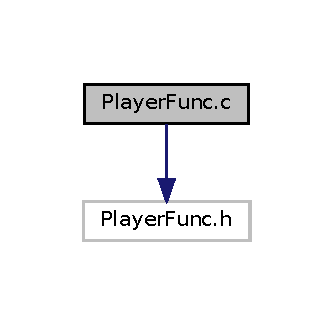
\includegraphics[width=160pt]{PlayerFunc_8c__incl}
\end{center}
\end{figure}
\subsection*{Functions}
\begin{DoxyCompactItemize}
\item 
Base $\ast$ \mbox{\hyperlink{PlayerFunc_8c_aaced0bd3de4e9bfdff0f9cc578f38973}{set\+Base\+Att}} (Base $\ast$bc, int x, int y, int height, int width)
\begin{DoxyCompactList}\small\item\em Função\+: Setar Atributos da Base. \end{DoxyCompactList}\item 
Build $\ast$ \mbox{\hyperlink{PlayerFunc_8c_a4d9be44221b41b95231736f3ead1f8e3}{set\+Build\+Att}} (Build $\ast$b, int x, int y, int height, int width, int type)
\begin{DoxyCompactList}\small\item\em Função\+: Setar Atributos dos Prédios. \end{DoxyCompactList}\item 
Troop $\ast$ \mbox{\hyperlink{PlayerFunc_8c_a4aa33629a3ca0e352afc8495c8fe7a9d}{set\+Troop\+Att}} (Troop $\ast$t, int x, int y, int type)
\begin{DoxyCompactList}\small\item\em Função\+: Setar Atributos das Tropas. \end{DoxyCompactList}\item 
void \mbox{\hyperlink{PlayerFunc_8c_a3d413144b7a4c3705c290f046df7262e}{move\+Troop}} (W\+I\+N\+D\+OW $\ast$win, char $\ast$$\ast$map)
\begin{DoxyCompactList}\small\item\em Função\+: Mover as Tropas. \end{DoxyCompactList}\item 
void \mbox{\hyperlink{PlayerFunc_8c_a32d049b69cc3b29b238d5f0d1e55235c}{resource\+Controller}} (Base $\ast$b, Build $\ast$b1, Build $\ast$b2)
\begin{DoxyCompactList}\small\item\em Função\+: Controlar a Mineração de Recursos. \end{DoxyCompactList}\item 
void \mbox{\hyperlink{PlayerFunc_8c_a6f112c057d34d8833d6cab06bb8c6a17}{troop\+Controller}} (Troop $\ast$t1, Troop $\ast$t2, Troop $\ast$t3, Build $\ast$b3, Base $\ast$b)
\begin{DoxyCompactList}\small\item\em Função\+: Controlar a Criação de Tropas. \end{DoxyCompactList}\item 
int \mbox{\hyperlink{PlayerFunc_8c_ab33aaf90543d021261eb4c9037921a2d}{troop\+Checker}} (Troop $\ast$t, int mode)
\begin{DoxyCompactList}\small\item\em Função\+: Verificar as Redondezas da Tropa. \end{DoxyCompactList}\item 
void \mbox{\hyperlink{PlayerFunc_8c_aefef57907035f8c1d6da57853beddc32}{build\+H\+P\+Checker}} (Build $\ast$b1, Build $\ast$b2, Build $\ast$b3, char $\ast$$\ast$map)
\begin{DoxyCompactList}\small\item\em Função\+: Verificar se um Prédio foi Derrubado. \end{DoxyCompactList}\item 
void \mbox{\hyperlink{PlayerFunc_8c_ae59ccce8fee4d7d21655f7747f766128}{troop\+Amount\+Checker}} (Troop $\ast$t1, Troop $\ast$t2, Troop $\ast$t3, char $\ast$$\ast$map)
\begin{DoxyCompactList}\small\item\em Função\+: Verificar se uma Tropa foi eliminada. \end{DoxyCompactList}\item 
void \mbox{\hyperlink{PlayerFunc_8c_ac5eb3097f64dc5e595b0eb00348dc70a}{battle\+Checker}} (Troop $\ast$t, Troop $\ast$t1\+\_\+e, Troop $\ast$t2\+\_\+e, Troop $\ast$t3\+\_\+e)
\begin{DoxyCompactList}\small\item\em Função\+: Controlar o Sistema de Batalha das Tropas. \end{DoxyCompactList}\item 
void \mbox{\hyperlink{PlayerFunc_8c_af0cfc04a4a66b4a70b4d9cad873aff1c}{destroy\+Build\+Checker}} (Troop $\ast$t, Base $\ast$b, Build $\ast$b1, Build $\ast$b2, Build $\ast$b3)
\begin{DoxyCompactList}\small\item\em Função\+: Controlar o Ataque de Tropas aos Prédios/\+Base. \end{DoxyCompactList}\end{DoxyCompactItemize}
\subsection*{Variables}
\begin{DoxyCompactItemize}
\item 
Base \mbox{\hyperlink{PlayerFunc_8c_aec091722f35907329e67f46c3161acdf}{Base\+\_\+p}}
\item 
Build \mbox{\hyperlink{PlayerFunc_8c_a925abcdbb079393da1518cec5b3ec5e1}{B1\+\_\+p}}
\item 
Build \mbox{\hyperlink{PlayerFunc_8c_ae38d253db63d8d5630d76742bea4e9eb}{B2\+\_\+p}}
\item 
Build \mbox{\hyperlink{PlayerFunc_8c_a3a341c97721e783906c060add6cf918e}{B3\+\_\+p}}
\item 
Troop \mbox{\hyperlink{PlayerFunc_8c_a77c37b243793bbcf4e14dcae4bdcf5b8}{T1\+\_\+p}}
\item 
Troop \mbox{\hyperlink{PlayerFunc_8c_ab0818f20f9722834079abffd7730c563}{T2\+\_\+p}}
\item 
Troop \mbox{\hyperlink{PlayerFunc_8c_a5815e52c3b85542221cef33fe258bc09}{T3\+\_\+p}}
\item 
int \mbox{\hyperlink{PlayerFunc_8c_ab0fb07f4c546cadaadff39b142526c6b}{troop\+Sel}} = 45
\end{DoxyCompactItemize}


\subsection{Function Documentation}
\mbox{\Hypertarget{PlayerFunc_8c_ac5eb3097f64dc5e595b0eb00348dc70a}\label{PlayerFunc_8c_ac5eb3097f64dc5e595b0eb00348dc70a}} 
\index{Player\+Func.\+c@{Player\+Func.\+c}!battle\+Checker@{battle\+Checker}}
\index{battle\+Checker@{battle\+Checker}!Player\+Func.\+c@{Player\+Func.\+c}}
\subsubsection{\texorpdfstring{battle\+Checker()}{battleChecker()}}
{\footnotesize\ttfamily void battle\+Checker (\begin{DoxyParamCaption}\item[{Troop $\ast$}]{t,  }\item[{Troop $\ast$}]{t1\+\_\+e,  }\item[{Troop $\ast$}]{t2\+\_\+e,  }\item[{Troop $\ast$}]{t3\+\_\+e }\end{DoxyParamCaption})}



Função\+: Controlar o Sistema de Batalha das Tropas. 

Descrição\+: A Função recebe as structs de uma das tropas do player de todas as tropas do PC. Então ela verifica de qual tropa do PC a tropa do player está do lado. De acordo com os atributos da tropa do player e da tropa do PC que ele está batalhando é calculado se as tropas do PC ou do Player diminuem. A tropa que ganhar a batalha vai perdendo seu número de tropas até chegar a 0 e sumir.

Parâmetros\+: 
\begin{DoxyParams}{Parameters}
{\em Troop$\ast$} & t -\/ struct da tropa do player \\
\hline
{\em Troop$\ast$} & t1\+\_\+e -\/ struct da tropa do tipo 1 do PC \\
\hline
{\em Troop$\ast$} & t2\+\_\+e -\/ struct da tropa do tipo 2 do PC \\
\hline
{\em Troop$\ast$} & b3 -\/ struct da tropa do tipo 3 do PC\\
\hline
\end{DoxyParams}
Valor retornado\+: \begin{DoxyReturn}{Returns}
Void. A função não retorna nada
\end{DoxyReturn}
Assertiva de entrada\+: Troop$\ast$ t != N\+U\+LL Troop$\ast$ t1\+\_\+e != N\+U\+LL Troop$\ast$ t2\+\_\+e != N\+U\+LL Troop$\ast$ t3\+\_\+e != N\+U\+LL

Assertiva de saída\+: Função void \mbox{\Hypertarget{PlayerFunc_8c_aefef57907035f8c1d6da57853beddc32}\label{PlayerFunc_8c_aefef57907035f8c1d6da57853beddc32}} 
\index{Player\+Func.\+c@{Player\+Func.\+c}!build\+H\+P\+Checker@{build\+H\+P\+Checker}}
\index{build\+H\+P\+Checker@{build\+H\+P\+Checker}!Player\+Func.\+c@{Player\+Func.\+c}}
\subsubsection{\texorpdfstring{build\+H\+P\+Checker()}{buildHPChecker()}}
{\footnotesize\ttfamily void build\+H\+P\+Checker (\begin{DoxyParamCaption}\item[{Build $\ast$}]{b1,  }\item[{Build $\ast$}]{b2,  }\item[{Build $\ast$}]{b3,  }\item[{char $\ast$$\ast$}]{map }\end{DoxyParamCaption})}



Função\+: Verificar se um Prédio foi Derrubado. 

Descrição\+: A Função recebe as structs dos prédios e a matriz do mapa. Ela verifica se a vida dos prédios é 0. Se for ela retira o prédio do mapa e deixa o hp da base como -\/1.

Parâmetros\+: 
\begin{DoxyParams}{Parameters}
{\em Build$\ast$} & b1 -\/ struct do prédio do tipo 1 \\
\hline
{\em Build$\ast$} & b2 -\/ struct do prédio do tipo 2 \\
\hline
{\em Build$\ast$} & b3 -\/ struct do prédio do tipo 3 \\
\hline
{\em char$\ast$$\ast$} & map -\/ matriz do mapa do jogo\\
\hline
\end{DoxyParams}
Valor retornado\+: \begin{DoxyReturn}{Returns}
Void. A função não retorna nada
\end{DoxyReturn}
Assertiva de entrada\+: Build$\ast$ b1 != N\+U\+LL Build$\ast$ b2 != N\+U\+LL Build$\ast$ b3 != N\+U\+LL Build$\ast$ b3 != N\+U\+LL char$\ast$$\ast$ map != N\+U\+LL

Assertiva de saída\+: Função void \mbox{\Hypertarget{PlayerFunc_8c_af0cfc04a4a66b4a70b4d9cad873aff1c}\label{PlayerFunc_8c_af0cfc04a4a66b4a70b4d9cad873aff1c}} 
\index{Player\+Func.\+c@{Player\+Func.\+c}!destroy\+Build\+Checker@{destroy\+Build\+Checker}}
\index{destroy\+Build\+Checker@{destroy\+Build\+Checker}!Player\+Func.\+c@{Player\+Func.\+c}}
\subsubsection{\texorpdfstring{destroy\+Build\+Checker()}{destroyBuildChecker()}}
{\footnotesize\ttfamily void destroy\+Build\+Checker (\begin{DoxyParamCaption}\item[{Troop $\ast$}]{t,  }\item[{Base $\ast$}]{b,  }\item[{Build $\ast$}]{b1,  }\item[{Build $\ast$}]{b2,  }\item[{Build $\ast$}]{b3 }\end{DoxyParamCaption})}



Função\+: Controlar o Ataque de Tropas aos Prédios/\+Base. 

Descrição\+: A Função recebe as structs dos prédios, da base e de uma tropa. Ela verifica se a tropa está perto de algum prédio/base e se estiver é calculado o dano que essa tropa está dando no prédio/base. Antes de diminuir a vida do prédio/base é necessário diminuir a defesa para 0.

Parâmetros\+: 
\begin{DoxyParams}{Parameters}
{\em Troop$\ast$} & t -\/ struct da tropa do tipo 1 \\
\hline
{\em Base$\ast$} & b -\/ struct da base \\
\hline
{\em Build$\ast$} & b1 -\/ struct do prédio do tipo 1 \\
\hline
{\em Build$\ast$} & b2 -\/ struct do prédio do tipo 2 \\
\hline
{\em Build$\ast$} & b3 -\/ struct do prédio do tipo 3\\
\hline
\end{DoxyParams}
Valor retornado\+: \begin{DoxyReturn}{Returns}
Void. A função não retorna nada
\end{DoxyReturn}
Assertiva de entrada\+: Troop$\ast$ t != N\+U\+LL Base$\ast$ b != N\+U\+LL Build$\ast$ b1 != N\+U\+LL Build$\ast$ b2 != N\+U\+LL Build$\ast$ b3 != N\+U\+LL

Assertiva de saída\+: Função void \mbox{\Hypertarget{PlayerFunc_8c_a3d413144b7a4c3705c290f046df7262e}\label{PlayerFunc_8c_a3d413144b7a4c3705c290f046df7262e}} 
\index{Player\+Func.\+c@{Player\+Func.\+c}!move\+Troop@{move\+Troop}}
\index{move\+Troop@{move\+Troop}!Player\+Func.\+c@{Player\+Func.\+c}}
\subsubsection{\texorpdfstring{move\+Troop()}{moveTroop()}}
{\footnotesize\ttfamily void move\+Troop (\begin{DoxyParamCaption}\item[{W\+I\+N\+D\+OW $\ast$}]{win,  }\item[{char $\ast$$\ast$}]{map }\end{DoxyParamCaption})}



Função\+: Mover as Tropas. 

Descrição\+: A Função recebe uma janela (ncurses) e uma matriz do mapa. Então ela verifica as entradas digitadas pelo usuário. No caso, 0, 1 e 2 para selecionar as tropas e/ou as teclas direcionais do teclado para movimentar as tropas. Então a função modifica a localização da tropa.

Parâmetros\+: 
\begin{DoxyParams}{Parameters}
{\em W\+I\+N\+D\+O\+W$\ast$} & win -\/ uma janela \\
\hline
{\em char$\ast$$\ast$} & map -\/ uma matriz que contém o mapa\\
\hline
\end{DoxyParams}
Valor retornado\+: \begin{DoxyReturn}{Returns}
Void -\/ a função não retorna nada
\end{DoxyReturn}
Assertiva de entrada\+: char$\ast$$\ast$ map != N\+U\+LL

Assertiva de saída\+: Função void \mbox{\Hypertarget{PlayerFunc_8c_a32d049b69cc3b29b238d5f0d1e55235c}\label{PlayerFunc_8c_a32d049b69cc3b29b238d5f0d1e55235c}} 
\index{Player\+Func.\+c@{Player\+Func.\+c}!resource\+Controller@{resource\+Controller}}
\index{resource\+Controller@{resource\+Controller}!Player\+Func.\+c@{Player\+Func.\+c}}
\subsubsection{\texorpdfstring{resource\+Controller()}{resourceController()}}
{\footnotesize\ttfamily void resource\+Controller (\begin{DoxyParamCaption}\item[{Base $\ast$}]{b,  }\item[{Build $\ast$}]{b1,  }\item[{Build $\ast$}]{b2 }\end{DoxyParamCaption})}



Função\+: Controlar a Mineração de Recursos. 

Descrição\+: A Função recebe as structs da base e de 2 prédios responsáveis pela mineração de recursos. Para controlar a frequencia de mineração, é verificado randomicamente um valor inteiro, e se ele for maior que 60 e a vida do prédio for superior a 0 é aumentado a quantidade de recursos minerados de acordo com a velocidade de mineração de cada tipo de prédio.

Parâmetros\+: 
\begin{DoxyParams}{Parameters}
{\em Base$\ast$} & b -\/ struct da base \\
\hline
{\em Build$\ast$} & b1 -\/ struct do prédio do tipo 1 \\
\hline
{\em Build$\ast$} & b2 -\/ struct do prédio do tipo 2\\
\hline
\end{DoxyParams}
Valor retornado\+: \begin{DoxyReturn}{Returns}
Void. A função não retorna nada
\end{DoxyReturn}
Assertiva de entrada\+: Base$\ast$ b != N\+U\+LL Build$\ast$ b1 != N\+U\+LL Build$\ast$ b2 != N\+U\+LL

Assertiva de saída\+: Função void \mbox{\Hypertarget{PlayerFunc_8c_aaced0bd3de4e9bfdff0f9cc578f38973}\label{PlayerFunc_8c_aaced0bd3de4e9bfdff0f9cc578f38973}} 
\index{Player\+Func.\+c@{Player\+Func.\+c}!set\+Base\+Att@{set\+Base\+Att}}
\index{set\+Base\+Att@{set\+Base\+Att}!Player\+Func.\+c@{Player\+Func.\+c}}
\subsubsection{\texorpdfstring{set\+Base\+Att()}{setBaseAtt()}}
{\footnotesize\ttfamily Base$\ast$ set\+Base\+Att (\begin{DoxyParamCaption}\item[{Base $\ast$}]{bc,  }\item[{int}]{x,  }\item[{int}]{y,  }\item[{int}]{height,  }\item[{int}]{width }\end{DoxyParamCaption})}



Função\+: Setar Atributos da Base. 

Descrição\+: A Função recebe uma struct da base, sua posição, comprimento e largura.\+Então esses valores são setados nessa struct e é setado também a quantidade de recursos 1 e 2, a defesa e a vida dessa base.

Parâmetros\+: 
\begin{DoxyParams}{Parameters}
{\em Base$\ast$} & bc -\/ uma struct para a base \\
\hline
{\em int} & x -\/ coordenada x da base \\
\hline
{\em int} & y -\/ coordenada y da base \\
\hline
{\em int} & height -\/ altura da base \\
\hline
{\em int} & width -\/ largura da base\\
\hline
\end{DoxyParams}
Valor retornado\+: \begin{DoxyReturn}{Returns}
Base$\ast$ bc -\/ struct com os valores modificados e iniciados para o começo do jogo
\end{DoxyReturn}
Assertiva de entrada\+: Base$\ast$ bc != N\+U\+LL int x $>$= 0 int y $>$= 0 int height $>$ 0 int width $>$ 0

Assertiva de saída\+: Base$\ast$ bc != N\+U\+LL \mbox{\Hypertarget{PlayerFunc_8c_a4d9be44221b41b95231736f3ead1f8e3}\label{PlayerFunc_8c_a4d9be44221b41b95231736f3ead1f8e3}} 
\index{Player\+Func.\+c@{Player\+Func.\+c}!set\+Build\+Att@{set\+Build\+Att}}
\index{set\+Build\+Att@{set\+Build\+Att}!Player\+Func.\+c@{Player\+Func.\+c}}
\subsubsection{\texorpdfstring{set\+Build\+Att()}{setBuildAtt()}}
{\footnotesize\ttfamily Build$\ast$ set\+Build\+Att (\begin{DoxyParamCaption}\item[{Build $\ast$}]{b,  }\item[{int}]{x,  }\item[{int}]{y,  }\item[{int}]{height,  }\item[{int}]{width,  }\item[{int}]{type }\end{DoxyParamCaption})}



Função\+: Setar Atributos dos Prédios. 

Descrição\+: A Função recebe uma struct de um prédio, sua posição, comprimento, largura e um valor inteiro que define qual o seu tipo.\+Então esses valores são setados nessa struct e é setado também, dependendo do tipo, a defesa, a velocidade de mineração, o consumo de recursos e a vida.

Parâmetros\+: 
\begin{DoxyParams}{Parameters}
{\em Build$\ast$} & b -\/ uma struct para o prédio \\
\hline
{\em int} & x -\/ coordenada x do prédio \\
\hline
{\em int} & y -\/ coordenada y do prédio \\
\hline
{\em int} & height -\/ altura do prédio \\
\hline
{\em int} & width -\/ largura do prédio \\
\hline
{\em int} & type -\/ tipo de prédio\\
\hline
\end{DoxyParams}
Valor retornado\+: \begin{DoxyReturn}{Returns}
Build$\ast$ b -\/ struct com os valores modificados e iniciados para o começo do jogo
\end{DoxyReturn}
Assertiva de entrada\+: Build$\ast$ b != N\+U\+LL int x $>$= 0 int y $>$= 0 int height $>$ 0 int width $>$ 0 int type == 0 $\vert$$\vert$ type == 1 $\vert$$\vert$ type == 2

Assertiva de saída\+: Build$\ast$ b != N\+U\+LL \mbox{\Hypertarget{PlayerFunc_8c_a4aa33629a3ca0e352afc8495c8fe7a9d}\label{PlayerFunc_8c_a4aa33629a3ca0e352afc8495c8fe7a9d}} 
\index{Player\+Func.\+c@{Player\+Func.\+c}!set\+Troop\+Att@{set\+Troop\+Att}}
\index{set\+Troop\+Att@{set\+Troop\+Att}!Player\+Func.\+c@{Player\+Func.\+c}}
\subsubsection{\texorpdfstring{set\+Troop\+Att()}{setTroopAtt()}}
{\footnotesize\ttfamily Troop$\ast$ set\+Troop\+Att (\begin{DoxyParamCaption}\item[{Troop $\ast$}]{t,  }\item[{int}]{x,  }\item[{int}]{y,  }\item[{int}]{type }\end{DoxyParamCaption})}



Função\+: Setar Atributos das Tropas. 

Descrição\+: A Função recebe uma struct das tropas, a sua posição e um valor inteiro que define qual o seu tipo. Então esses valores,menos o tipo, são setados nessa struct e é setado também, dependendo do seu tipo, quantidade de soldados na tropa, o dano da tropa, a defesa da tropa e a sua vida.

Parâmetros\+: 
\begin{DoxyParams}{Parameters}
{\em Troop$\ast$} & bc -\/ uma struct para a tropa \\
\hline
{\em int} & x -\/ coordenada x da tropa \\
\hline
{\em int} & y -\/ coordenada y da tropa \\
\hline
{\em int} & type -\/ tipo de tropa\\
\hline
\end{DoxyParams}
Valor retornado\+: \begin{DoxyReturn}{Returns}
Troop$\ast$ t -\/ struct com os valores modificados e iniciados para o começo do jogo
\end{DoxyReturn}
Assertiva de entrada\+: Troop$\ast$ t != N\+U\+LL int x $>$= 0 int y $>$= 0 int type == 0 $\vert$$\vert$ type == 1 $\vert$$\vert$ type == 2

Assertiva de saída\+: Troop$\ast$ t != N\+U\+LL \mbox{\Hypertarget{PlayerFunc_8c_ae59ccce8fee4d7d21655f7747f766128}\label{PlayerFunc_8c_ae59ccce8fee4d7d21655f7747f766128}} 
\index{Player\+Func.\+c@{Player\+Func.\+c}!troop\+Amount\+Checker@{troop\+Amount\+Checker}}
\index{troop\+Amount\+Checker@{troop\+Amount\+Checker}!Player\+Func.\+c@{Player\+Func.\+c}}
\subsubsection{\texorpdfstring{troop\+Amount\+Checker()}{troopAmountChecker()}}
{\footnotesize\ttfamily void troop\+Amount\+Checker (\begin{DoxyParamCaption}\item[{Troop $\ast$}]{t1,  }\item[{Troop $\ast$}]{t2,  }\item[{Troop $\ast$}]{t3,  }\item[{char $\ast$$\ast$}]{map }\end{DoxyParamCaption})}



Função\+: Verificar se uma Tropa foi eliminada. 

Descrição\+: A Função recebe as structs das tropas e a matriz do mapa. Ela verifica se a quantidade de tropas é igual a zero e se for ela retira a tropa do mapa.

Parâmetros\+: 
\begin{DoxyParams}{Parameters}
{\em Troop$\ast$} & t1 -\/ struct da tropa do tipo 1 \\
\hline
{\em Troop$\ast$} & t2 -\/ struct da tropa do tipo 2 \\
\hline
{\em Troop$\ast$} & t3 -\/ struct da tropa do tipo 3 \\
\hline
{\em char$\ast$$\ast$} & map -\/ matriz do mapa\\
\hline
\end{DoxyParams}
Valor retornado\+: \begin{DoxyReturn}{Returns}
Void. A função não retorna nada
\end{DoxyReturn}
Assertiva de entrada\+: Troop$\ast$ t1 != N\+U\+LL Troop$\ast$ t2 != N\+U\+LL Troop$\ast$ t3 != N\+U\+LL char$\ast$$\ast$ map != N\+U\+LL

Assertiva de saída\+: Função void \mbox{\Hypertarget{PlayerFunc_8c_ab33aaf90543d021261eb4c9037921a2d}\label{PlayerFunc_8c_ab33aaf90543d021261eb4c9037921a2d}} 
\index{Player\+Func.\+c@{Player\+Func.\+c}!troop\+Checker@{troop\+Checker}}
\index{troop\+Checker@{troop\+Checker}!Player\+Func.\+c@{Player\+Func.\+c}}
\subsubsection{\texorpdfstring{troop\+Checker()}{troopChecker()}}
{\footnotesize\ttfamily int troop\+Checker (\begin{DoxyParamCaption}\item[{Troop $\ast$}]{t,  }\item[{int}]{mode }\end{DoxyParamCaption})}



Função\+: Verificar as Redondezas da Tropa. 

Descrição\+: A Função recebe a struct de uma tropa e verifica as redondezas dessa tropa, e retorna um valor de acordo com o que está do lado dessa tropa.

Parâmetros\+: 
\begin{DoxyParams}{Parameters}
{\em Troop$\ast$} & t -\/ struct da tropa \\
\hline
{\em int} & mode -\/ flag para identificar se a função foi chamada para checar se a tropa está perto do prédio responsável por aumentar tropas (0) ou se foi chamada para checar se há tropas inimigas por perto (1)\\
\hline
\end{DoxyParams}
Valor retornado\+: \begin{DoxyReturn}{Returns}
0 -\/ caso a tropa não esteja perto de nada 

1 -\/ caso a mode = 0 e a tropa esteja perto do prédio responsável por gerar tropas 

7 -\/ caso a tropa esteja perto da tropa inimiga \textquotesingle{}7\textquotesingle{} 

8 -\/ caso a tropa esteja perto da tropa inimiga \textquotesingle{}8\textquotesingle{} 

9 -\/ caso a tropa esteja perto da tropa inimiga \textquotesingle{}9\textquotesingle{} 

10 -\/ caso a tropa esteja perto do base \textquotesingle{}Y\textquotesingle{} 

11 -\/ caso a tropa esteja perto do prédio \textquotesingle{}D\textquotesingle{} 

12 -\/ caso a tropa esteja perto do prédio \textquotesingle{}F\textquotesingle{} 

13 -\/ caso a tropa esteja perto do prédio \textquotesingle{}E\textquotesingle{}
\end{DoxyReturn}
Assertiva de entrada\+: Troop$\ast$ t != N\+U\+LL int mode == 0 $\vert$$\vert$ mode == 1

Assertiva de saída\+: A função retorna valores fixos. \mbox{\Hypertarget{PlayerFunc_8c_a6f112c057d34d8833d6cab06bb8c6a17}\label{PlayerFunc_8c_a6f112c057d34d8833d6cab06bb8c6a17}} 
\index{Player\+Func.\+c@{Player\+Func.\+c}!troop\+Controller@{troop\+Controller}}
\index{troop\+Controller@{troop\+Controller}!Player\+Func.\+c@{Player\+Func.\+c}}
\subsubsection{\texorpdfstring{troop\+Controller()}{troopController()}}
{\footnotesize\ttfamily void troop\+Controller (\begin{DoxyParamCaption}\item[{Troop $\ast$}]{t1,  }\item[{Troop $\ast$}]{t2,  }\item[{Troop $\ast$}]{t3,  }\item[{Build $\ast$}]{b3,  }\item[{Base $\ast$}]{b }\end{DoxyParamCaption})}



Função\+: Controlar a Criação de Tropas. 

Descrição\+: A Função recebe as structs da base, das tropas e do prédio responsável pela criação de tropas. Então ela verifica se a tropa está do lado do prédio que gera tropa, e se há recursos para gerar mais tropas. Então essa tropa tem a quantidade aumentada.

Parâmetros\+: 
\begin{DoxyParams}{Parameters}
{\em Troop$\ast$} & t1 -\/ struct da tropa do tipo 1 \\
\hline
{\em Troop$\ast$} & t2 -\/ struct da tropa do tipo 2 \\
\hline
{\em Troop$\ast$} & t3 -\/ struct da tropa do tipo 3 \\
\hline
{\em Build$\ast$} & b3 -\/ struct do prédio do tipo 3 \\
\hline
{\em Base$\ast$} & b -\/ struct da base\\
\hline
\end{DoxyParams}
Valor retornado\+: \begin{DoxyReturn}{Returns}
Void. A função não retorna nada
\end{DoxyReturn}
Assertiva de entrada\+: Troop$\ast$ t1 != N\+U\+LL Troop$\ast$ t2 != N\+U\+LL Troop$\ast$ t3 != N\+U\+LL Build$\ast$ b3 != N\+U\+LL Base$\ast$ b != N\+U\+LL

Assertiva de saída\+: Função void 

\subsection{Variable Documentation}
\mbox{\Hypertarget{PlayerFunc_8c_a925abcdbb079393da1518cec5b3ec5e1}\label{PlayerFunc_8c_a925abcdbb079393da1518cec5b3ec5e1}} 
\index{Player\+Func.\+c@{Player\+Func.\+c}!B1\+\_\+p@{B1\+\_\+p}}
\index{B1\+\_\+p@{B1\+\_\+p}!Player\+Func.\+c@{Player\+Func.\+c}}
\subsubsection{\texorpdfstring{B1\+\_\+p}{B1\_p}}
{\footnotesize\ttfamily Build B1\+\_\+p}

struct prédio 1 \mbox{\Hypertarget{PlayerFunc_8c_ae38d253db63d8d5630d76742bea4e9eb}\label{PlayerFunc_8c_ae38d253db63d8d5630d76742bea4e9eb}} 
\index{Player\+Func.\+c@{Player\+Func.\+c}!B2\+\_\+p@{B2\+\_\+p}}
\index{B2\+\_\+p@{B2\+\_\+p}!Player\+Func.\+c@{Player\+Func.\+c}}
\subsubsection{\texorpdfstring{B2\+\_\+p}{B2\_p}}
{\footnotesize\ttfamily Build B2\+\_\+p}

struct prédio 2 \mbox{\Hypertarget{PlayerFunc_8c_a3a341c97721e783906c060add6cf918e}\label{PlayerFunc_8c_a3a341c97721e783906c060add6cf918e}} 
\index{Player\+Func.\+c@{Player\+Func.\+c}!B3\+\_\+p@{B3\+\_\+p}}
\index{B3\+\_\+p@{B3\+\_\+p}!Player\+Func.\+c@{Player\+Func.\+c}}
\subsubsection{\texorpdfstring{B3\+\_\+p}{B3\_p}}
{\footnotesize\ttfamily Build B3\+\_\+p}

struct prédio 3 \mbox{\Hypertarget{PlayerFunc_8c_aec091722f35907329e67f46c3161acdf}\label{PlayerFunc_8c_aec091722f35907329e67f46c3161acdf}} 
\index{Player\+Func.\+c@{Player\+Func.\+c}!Base\+\_\+p@{Base\+\_\+p}}
\index{Base\+\_\+p@{Base\+\_\+p}!Player\+Func.\+c@{Player\+Func.\+c}}
\subsubsection{\texorpdfstring{Base\+\_\+p}{Base\_p}}
{\footnotesize\ttfamily Base Base\+\_\+p}

struct base \mbox{\Hypertarget{PlayerFunc_8c_a77c37b243793bbcf4e14dcae4bdcf5b8}\label{PlayerFunc_8c_a77c37b243793bbcf4e14dcae4bdcf5b8}} 
\index{Player\+Func.\+c@{Player\+Func.\+c}!T1\+\_\+p@{T1\+\_\+p}}
\index{T1\+\_\+p@{T1\+\_\+p}!Player\+Func.\+c@{Player\+Func.\+c}}
\subsubsection{\texorpdfstring{T1\+\_\+p}{T1\_p}}
{\footnotesize\ttfamily Troop T1\+\_\+p}

struct tropa 1 \mbox{\Hypertarget{PlayerFunc_8c_ab0818f20f9722834079abffd7730c563}\label{PlayerFunc_8c_ab0818f20f9722834079abffd7730c563}} 
\index{Player\+Func.\+c@{Player\+Func.\+c}!T2\+\_\+p@{T2\+\_\+p}}
\index{T2\+\_\+p@{T2\+\_\+p}!Player\+Func.\+c@{Player\+Func.\+c}}
\subsubsection{\texorpdfstring{T2\+\_\+p}{T2\_p}}
{\footnotesize\ttfamily Troop T2\+\_\+p}

struct tropa 2 \mbox{\Hypertarget{PlayerFunc_8c_a5815e52c3b85542221cef33fe258bc09}\label{PlayerFunc_8c_a5815e52c3b85542221cef33fe258bc09}} 
\index{Player\+Func.\+c@{Player\+Func.\+c}!T3\+\_\+p@{T3\+\_\+p}}
\index{T3\+\_\+p@{T3\+\_\+p}!Player\+Func.\+c@{Player\+Func.\+c}}
\subsubsection{\texorpdfstring{T3\+\_\+p}{T3\_p}}
{\footnotesize\ttfamily Troop T3\+\_\+p}

struct tropa 3 \mbox{\Hypertarget{PlayerFunc_8c_ab0fb07f4c546cadaadff39b142526c6b}\label{PlayerFunc_8c_ab0fb07f4c546cadaadff39b142526c6b}} 
\index{Player\+Func.\+c@{Player\+Func.\+c}!troop\+Sel@{troop\+Sel}}
\index{troop\+Sel@{troop\+Sel}!Player\+Func.\+c@{Player\+Func.\+c}}
\subsubsection{\texorpdfstring{troop\+Sel}{troopSel}}
{\footnotesize\ttfamily int troop\+Sel = 45}

variável que mostra qual tropa está selecionada 
\hypertarget{Tests_8c}{}\section{Tests.\+c File Reference}
\label{Tests_8c}\index{Tests.\+c@{Tests.\+c}}
{\ttfamily \#include \char`\"{}Win\+Manager.\+h\char`\"{}}\newline
{\ttfamily \#include \char`\"{}C\+Unit/\+Basic.\+h\char`\"{}}\newline
Include dependency graph for Tests.\+c\+:
\nopagebreak
\begin{figure}[H]
\begin{center}
\leavevmode
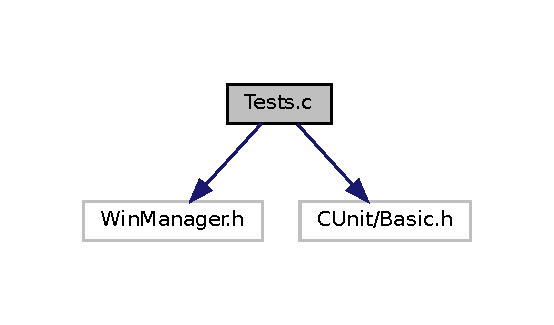
\includegraphics[width=266pt]{Tests_8c__incl}
\end{center}
\end{figure}
\subsection*{Functions}
\begin{DoxyCompactItemize}
\item 
void \mbox{\hyperlink{Tests_8c_a2988c145e945445e942d63f19cb509fa}{test\+A\+L\+L\+O\+C\+M\+AP}} (void)
\item 
void \mbox{\hyperlink{Tests_8c_a32f034f7f599cad68773bac942580620}{test\+D\+E\+A\+L\+L\+O\+C\+M\+AP}} (void)
\item 
void \mbox{\hyperlink{Tests_8c_aece834ec508de38109b6ab0bff7ee0a6}{test\+S\+E\+T\+B\+A\+S\+E\+O\+N\+M\+AP}} (void)
\item 
void \mbox{\hyperlink{Tests_8c_ad5f8d2e1869447d1cec623b462c1e930}{test\+S\+E\+T\+B\+U\+I\+L\+D\+O\+N\+M\+AP}} (void)
\item 
void \mbox{\hyperlink{Tests_8c_a44bd30704af30429eb70c26dbd3b1896}{test\+S\+E\+T\+T\+R\+O\+O\+P\+O\+N\+M\+AP}} (void)
\item 
void \mbox{\hyperlink{Tests_8c_a261233137ef393f0e1896aeb84d62d8d}{test\+S\+E\+T\+M\+AP}} (void)
\item 
void \mbox{\hyperlink{Tests_8c_a20f503e2f34193415cc0cd61c10772d4}{test\+S\+E\+T\+B\+A\+S\+E\+A\+TT}} (void)
\item 
void \mbox{\hyperlink{Tests_8c_a78d77dfa64360779177c9ab23688d5f8}{test\+S\+E\+T\+B\+U\+I\+L\+D\+A\+TT}} (void)
\item 
void \mbox{\hyperlink{Tests_8c_a16dc3e3e2749966d6fd8f0bacc088f06}{test\+S\+E\+T\+T\+R\+O\+O\+P\+A\+TT}} (void)
\item 
void \mbox{\hyperlink{Tests_8c_a7c4e72bd22b999abccff76add831e492}{test\+T\+R\+O\+O\+P\+C\+H\+E\+C\+K\+ER}} (void)
\item 
void \mbox{\hyperlink{Tests_8c_a289e00b528cfece9a2722a314559ae5a}{test\+T\+R\+O\+O\+P\+C\+O\+N\+T\+R\+O\+L\+L\+ER}} (void)
\item 
void \mbox{\hyperlink{Tests_8c_ab2a3c491c0c7d5f172fca1bd7f90b8fd}{test\+B\+U\+I\+L\+D\+H\+P\+C\+H\+E\+C\+K\+ER}} (void)
\item 
void \mbox{\hyperlink{Tests_8c_aa523bca7750d46af014351344353b7d6}{test\+T\+R\+O\+O\+P\+A\+M\+O\+U\+N\+T\+C\+H\+E\+C\+K\+ER}} (void)
\item 
void \mbox{\hyperlink{Tests_8c_a7de6dc0c602e070252b2920fe31c6a93}{test\+B\+A\+T\+T\+L\+E\+C\+H\+E\+C\+K\+ER}} (void)
\item 
void \mbox{\hyperlink{Tests_8c_ab409af1ed33efcf4706d6fe64af6cd18}{test\+D\+E\+S\+T\+R\+O\+Y\+B\+U\+I\+L\+D\+C\+H\+E\+C\+K\+ER}} (void)
\item 
void \mbox{\hyperlink{Tests_8c_a2472209a95e0fe0c3643ad9e3eaa075e}{test\+L\+O\+A\+D\+G\+A\+ME}} (void)
\item 
void \mbox{\hyperlink{Tests_8c_ab549ee7e66eb0426152d2165f79462aa}{test\+E\+N\+E\+M\+Y\+T\+R\+O\+O\+P\+C\+H\+E\+C\+K\+ER}} (void)
\item 
void \mbox{\hyperlink{Tests_8c_aee46f24337ca86a200f7d5209f321d31}{test\+E\+N\+E\+M\+Y\+T\+R\+O\+O\+P\+C\+O\+N\+T\+R\+O\+L\+L\+ER}} (void)
\item 
void \mbox{\hyperlink{Tests_8c_a815a418217292e648342f013339bce40}{test\+E\+N\+E\+M\+Y\+H\+I\+T\+C\+O\+N\+T\+R\+OL}} (void)
\item 
int \mbox{\hyperlink{Tests_8c_a736aee61f9f1e8c0ba3aa9734cd13b5d}{init\+\_\+suite1}} (void)
\item 
int \mbox{\hyperlink{Tests_8c_ac8dcdd2549f2c6bee1c950bb827b8347}{clean\+\_\+suite1}} (void)
\item 
int \mbox{\hyperlink{Tests_8c_ae66f6b31b5ad750f1fe042a706a4e3d4}{main}} ()
\end{DoxyCompactItemize}


\subsection{Function Documentation}
\mbox{\Hypertarget{Tests_8c_ac8dcdd2549f2c6bee1c950bb827b8347}\label{Tests_8c_ac8dcdd2549f2c6bee1c950bb827b8347}} 
\index{Tests.\+c@{Tests.\+c}!clean\+\_\+suite1@{clean\+\_\+suite1}}
\index{clean\+\_\+suite1@{clean\+\_\+suite1}!Tests.\+c@{Tests.\+c}}
\subsubsection{\texorpdfstring{clean\+\_\+suite1()}{clean\_suite1()}}
{\footnotesize\ttfamily int clean\+\_\+suite1 (\begin{DoxyParamCaption}\item[{void}]{ }\end{DoxyParamCaption})}

The suite cleanup function. Closes the temporary file used by the tests. Returns zero on success, non-\/zero otherwise. \mbox{\Hypertarget{Tests_8c_a736aee61f9f1e8c0ba3aa9734cd13b5d}\label{Tests_8c_a736aee61f9f1e8c0ba3aa9734cd13b5d}} 
\index{Tests.\+c@{Tests.\+c}!init\+\_\+suite1@{init\+\_\+suite1}}
\index{init\+\_\+suite1@{init\+\_\+suite1}!Tests.\+c@{Tests.\+c}}
\subsubsection{\texorpdfstring{init\+\_\+suite1()}{init\_suite1()}}
{\footnotesize\ttfamily int init\+\_\+suite1 (\begin{DoxyParamCaption}\item[{void}]{ }\end{DoxyParamCaption})}

The suite initialization function. Opens the temporary file used by the tests. Returns zero on success, non-\/zero otherwise. \mbox{\Hypertarget{Tests_8c_ae66f6b31b5ad750f1fe042a706a4e3d4}\label{Tests_8c_ae66f6b31b5ad750f1fe042a706a4e3d4}} 
\index{Tests.\+c@{Tests.\+c}!main@{main}}
\index{main@{main}!Tests.\+c@{Tests.\+c}}
\subsubsection{\texorpdfstring{main()}{main()}}
{\footnotesize\ttfamily int main (\begin{DoxyParamCaption}{ }\end{DoxyParamCaption})}

\mbox{\Hypertarget{Tests_8c_a2988c145e945445e942d63f19cb509fa}\label{Tests_8c_a2988c145e945445e942d63f19cb509fa}} 
\index{Tests.\+c@{Tests.\+c}!test\+A\+L\+L\+O\+C\+M\+AP@{test\+A\+L\+L\+O\+C\+M\+AP}}
\index{test\+A\+L\+L\+O\+C\+M\+AP@{test\+A\+L\+L\+O\+C\+M\+AP}!Tests.\+c@{Tests.\+c}}
\subsubsection{\texorpdfstring{test\+A\+L\+L\+O\+C\+M\+A\+P()}{testALLOCMAP()}}
{\footnotesize\ttfamily void test\+A\+L\+L\+O\+C\+M\+AP (\begin{DoxyParamCaption}\item[{void}]{ }\end{DoxyParamCaption})}

Teste para verificar se o mapa aloca de forma correta \mbox{\Hypertarget{Tests_8c_a7de6dc0c602e070252b2920fe31c6a93}\label{Tests_8c_a7de6dc0c602e070252b2920fe31c6a93}} 
\index{Tests.\+c@{Tests.\+c}!test\+B\+A\+T\+T\+L\+E\+C\+H\+E\+C\+K\+ER@{test\+B\+A\+T\+T\+L\+E\+C\+H\+E\+C\+K\+ER}}
\index{test\+B\+A\+T\+T\+L\+E\+C\+H\+E\+C\+K\+ER@{test\+B\+A\+T\+T\+L\+E\+C\+H\+E\+C\+K\+ER}!Tests.\+c@{Tests.\+c}}
\subsubsection{\texorpdfstring{test\+B\+A\+T\+T\+L\+E\+C\+H\+E\+C\+K\+E\+R()}{testBATTLECHECKER()}}
{\footnotesize\ttfamily void test\+B\+A\+T\+T\+L\+E\+C\+H\+E\+C\+K\+ER (\begin{DoxyParamCaption}\item[{void}]{ }\end{DoxyParamCaption})}

Teste para verificar se as batalhas entre tropas funciona como o esperado \mbox{\Hypertarget{Tests_8c_ab2a3c491c0c7d5f172fca1bd7f90b8fd}\label{Tests_8c_ab2a3c491c0c7d5f172fca1bd7f90b8fd}} 
\index{Tests.\+c@{Tests.\+c}!test\+B\+U\+I\+L\+D\+H\+P\+C\+H\+E\+C\+K\+ER@{test\+B\+U\+I\+L\+D\+H\+P\+C\+H\+E\+C\+K\+ER}}
\index{test\+B\+U\+I\+L\+D\+H\+P\+C\+H\+E\+C\+K\+ER@{test\+B\+U\+I\+L\+D\+H\+P\+C\+H\+E\+C\+K\+ER}!Tests.\+c@{Tests.\+c}}
\subsubsection{\texorpdfstring{test\+B\+U\+I\+L\+D\+H\+P\+C\+H\+E\+C\+K\+E\+R()}{testBUILDHPCHECKER()}}
{\footnotesize\ttfamily void test\+B\+U\+I\+L\+D\+H\+P\+C\+H\+E\+C\+K\+ER (\begin{DoxyParamCaption}\item[{void}]{ }\end{DoxyParamCaption})}

Teste para verificar se os prédios são destruídos corretamente quando a vida deles chega a zero \mbox{\Hypertarget{Tests_8c_a32f034f7f599cad68773bac942580620}\label{Tests_8c_a32f034f7f599cad68773bac942580620}} 
\index{Tests.\+c@{Tests.\+c}!test\+D\+E\+A\+L\+L\+O\+C\+M\+AP@{test\+D\+E\+A\+L\+L\+O\+C\+M\+AP}}
\index{test\+D\+E\+A\+L\+L\+O\+C\+M\+AP@{test\+D\+E\+A\+L\+L\+O\+C\+M\+AP}!Tests.\+c@{Tests.\+c}}
\subsubsection{\texorpdfstring{test\+D\+E\+A\+L\+L\+O\+C\+M\+A\+P()}{testDEALLOCMAP()}}
{\footnotesize\ttfamily void test\+D\+E\+A\+L\+L\+O\+C\+M\+AP (\begin{DoxyParamCaption}\item[{void}]{ }\end{DoxyParamCaption})}

Teste para verificar se o mapa desaloca de forma correta \mbox{\Hypertarget{Tests_8c_ab409af1ed33efcf4706d6fe64af6cd18}\label{Tests_8c_ab409af1ed33efcf4706d6fe64af6cd18}} 
\index{Tests.\+c@{Tests.\+c}!test\+D\+E\+S\+T\+R\+O\+Y\+B\+U\+I\+L\+D\+C\+H\+E\+C\+K\+ER@{test\+D\+E\+S\+T\+R\+O\+Y\+B\+U\+I\+L\+D\+C\+H\+E\+C\+K\+ER}}
\index{test\+D\+E\+S\+T\+R\+O\+Y\+B\+U\+I\+L\+D\+C\+H\+E\+C\+K\+ER@{test\+D\+E\+S\+T\+R\+O\+Y\+B\+U\+I\+L\+D\+C\+H\+E\+C\+K\+ER}!Tests.\+c@{Tests.\+c}}
\subsubsection{\texorpdfstring{test\+D\+E\+S\+T\+R\+O\+Y\+B\+U\+I\+L\+D\+C\+H\+E\+C\+K\+E\+R()}{testDESTROYBUILDCHECKER()}}
{\footnotesize\ttfamily void test\+D\+E\+S\+T\+R\+O\+Y\+B\+U\+I\+L\+D\+C\+H\+E\+C\+K\+ER (\begin{DoxyParamCaption}\item[{void}]{ }\end{DoxyParamCaption})}

Teste para verificar se as tropas atacam da forma esperada a base e os prédios inimigos \mbox{\Hypertarget{Tests_8c_a815a418217292e648342f013339bce40}\label{Tests_8c_a815a418217292e648342f013339bce40}} 
\index{Tests.\+c@{Tests.\+c}!test\+E\+N\+E\+M\+Y\+H\+I\+T\+C\+O\+N\+T\+R\+OL@{test\+E\+N\+E\+M\+Y\+H\+I\+T\+C\+O\+N\+T\+R\+OL}}
\index{test\+E\+N\+E\+M\+Y\+H\+I\+T\+C\+O\+N\+T\+R\+OL@{test\+E\+N\+E\+M\+Y\+H\+I\+T\+C\+O\+N\+T\+R\+OL}!Tests.\+c@{Tests.\+c}}
\subsubsection{\texorpdfstring{test\+E\+N\+E\+M\+Y\+H\+I\+T\+C\+O\+N\+T\+R\+O\+L()}{testENEMYHITCONTROL()}}
{\footnotesize\ttfamily void test\+E\+N\+E\+M\+Y\+H\+I\+T\+C\+O\+N\+T\+R\+OL (\begin{DoxyParamCaption}\item[{void}]{ }\end{DoxyParamCaption})}

Teste para verificar se as tropas do PC atacam da forma esperada a base e os prédios do player \mbox{\Hypertarget{Tests_8c_ab549ee7e66eb0426152d2165f79462aa}\label{Tests_8c_ab549ee7e66eb0426152d2165f79462aa}} 
\index{Tests.\+c@{Tests.\+c}!test\+E\+N\+E\+M\+Y\+T\+R\+O\+O\+P\+C\+H\+E\+C\+K\+ER@{test\+E\+N\+E\+M\+Y\+T\+R\+O\+O\+P\+C\+H\+E\+C\+K\+ER}}
\index{test\+E\+N\+E\+M\+Y\+T\+R\+O\+O\+P\+C\+H\+E\+C\+K\+ER@{test\+E\+N\+E\+M\+Y\+T\+R\+O\+O\+P\+C\+H\+E\+C\+K\+ER}!Tests.\+c@{Tests.\+c}}
\subsubsection{\texorpdfstring{test\+E\+N\+E\+M\+Y\+T\+R\+O\+O\+P\+C\+H\+E\+C\+K\+E\+R()}{testENEMYTROOPCHECKER()}}
{\footnotesize\ttfamily void test\+E\+N\+E\+M\+Y\+T\+R\+O\+O\+P\+C\+H\+E\+C\+K\+ER (\begin{DoxyParamCaption}\item[{void}]{ }\end{DoxyParamCaption})}

Teste para verificar se a tropa do PC identifica quando atacar e quando está do lado de um prédio que aumenta tropas \mbox{\Hypertarget{Tests_8c_aee46f24337ca86a200f7d5209f321d31}\label{Tests_8c_aee46f24337ca86a200f7d5209f321d31}} 
\index{Tests.\+c@{Tests.\+c}!test\+E\+N\+E\+M\+Y\+T\+R\+O\+O\+P\+C\+O\+N\+T\+R\+O\+L\+L\+ER@{test\+E\+N\+E\+M\+Y\+T\+R\+O\+O\+P\+C\+O\+N\+T\+R\+O\+L\+L\+ER}}
\index{test\+E\+N\+E\+M\+Y\+T\+R\+O\+O\+P\+C\+O\+N\+T\+R\+O\+L\+L\+ER@{test\+E\+N\+E\+M\+Y\+T\+R\+O\+O\+P\+C\+O\+N\+T\+R\+O\+L\+L\+ER}!Tests.\+c@{Tests.\+c}}
\subsubsection{\texorpdfstring{test\+E\+N\+E\+M\+Y\+T\+R\+O\+O\+P\+C\+O\+N\+T\+R\+O\+L\+L\+E\+R()}{testENEMYTROOPCONTROLLER()}}
{\footnotesize\ttfamily void test\+E\+N\+E\+M\+Y\+T\+R\+O\+O\+P\+C\+O\+N\+T\+R\+O\+L\+L\+ER (\begin{DoxyParamCaption}\item[{void}]{ }\end{DoxyParamCaption})}

Teste para verificar se a tropa do PC é gerada de forma certa \mbox{\Hypertarget{Tests_8c_a2472209a95e0fe0c3643ad9e3eaa075e}\label{Tests_8c_a2472209a95e0fe0c3643ad9e3eaa075e}} 
\index{Tests.\+c@{Tests.\+c}!test\+L\+O\+A\+D\+G\+A\+ME@{test\+L\+O\+A\+D\+G\+A\+ME}}
\index{test\+L\+O\+A\+D\+G\+A\+ME@{test\+L\+O\+A\+D\+G\+A\+ME}!Tests.\+c@{Tests.\+c}}
\subsubsection{\texorpdfstring{test\+L\+O\+A\+D\+G\+A\+M\+E()}{testLOADGAME()}}
{\footnotesize\ttfamily void test\+L\+O\+A\+D\+G\+A\+ME (\begin{DoxyParamCaption}\item[{void}]{ }\end{DoxyParamCaption})}

Teste para verificar se o jogo lê o save de forma correta \mbox{\Hypertarget{Tests_8c_a20f503e2f34193415cc0cd61c10772d4}\label{Tests_8c_a20f503e2f34193415cc0cd61c10772d4}} 
\index{Tests.\+c@{Tests.\+c}!test\+S\+E\+T\+B\+A\+S\+E\+A\+TT@{test\+S\+E\+T\+B\+A\+S\+E\+A\+TT}}
\index{test\+S\+E\+T\+B\+A\+S\+E\+A\+TT@{test\+S\+E\+T\+B\+A\+S\+E\+A\+TT}!Tests.\+c@{Tests.\+c}}
\subsubsection{\texorpdfstring{test\+S\+E\+T\+B\+A\+S\+E\+A\+T\+T()}{testSETBASEATT()}}
{\footnotesize\ttfamily void test\+S\+E\+T\+B\+A\+S\+E\+A\+TT (\begin{DoxyParamCaption}\item[{void}]{ }\end{DoxyParamCaption})}

Teste para verificar se a Base é inicializada corretamente \mbox{\Hypertarget{Tests_8c_aece834ec508de38109b6ab0bff7ee0a6}\label{Tests_8c_aece834ec508de38109b6ab0bff7ee0a6}} 
\index{Tests.\+c@{Tests.\+c}!test\+S\+E\+T\+B\+A\+S\+E\+O\+N\+M\+AP@{test\+S\+E\+T\+B\+A\+S\+E\+O\+N\+M\+AP}}
\index{test\+S\+E\+T\+B\+A\+S\+E\+O\+N\+M\+AP@{test\+S\+E\+T\+B\+A\+S\+E\+O\+N\+M\+AP}!Tests.\+c@{Tests.\+c}}
\subsubsection{\texorpdfstring{test\+S\+E\+T\+B\+A\+S\+E\+O\+N\+M\+A\+P()}{testSETBASEONMAP()}}
{\footnotesize\ttfamily void test\+S\+E\+T\+B\+A\+S\+E\+O\+N\+M\+AP (\begin{DoxyParamCaption}\item[{void}]{ }\end{DoxyParamCaption})}

Teste para verificar se a base é colocada de forma correta no mapa \mbox{\Hypertarget{Tests_8c_a78d77dfa64360779177c9ab23688d5f8}\label{Tests_8c_a78d77dfa64360779177c9ab23688d5f8}} 
\index{Tests.\+c@{Tests.\+c}!test\+S\+E\+T\+B\+U\+I\+L\+D\+A\+TT@{test\+S\+E\+T\+B\+U\+I\+L\+D\+A\+TT}}
\index{test\+S\+E\+T\+B\+U\+I\+L\+D\+A\+TT@{test\+S\+E\+T\+B\+U\+I\+L\+D\+A\+TT}!Tests.\+c@{Tests.\+c}}
\subsubsection{\texorpdfstring{test\+S\+E\+T\+B\+U\+I\+L\+D\+A\+T\+T()}{testSETBUILDATT()}}
{\footnotesize\ttfamily void test\+S\+E\+T\+B\+U\+I\+L\+D\+A\+TT (\begin{DoxyParamCaption}\item[{void}]{ }\end{DoxyParamCaption})}

Teste para verificar se os Builds são inicializados corretamente \mbox{\Hypertarget{Tests_8c_ad5f8d2e1869447d1cec623b462c1e930}\label{Tests_8c_ad5f8d2e1869447d1cec623b462c1e930}} 
\index{Tests.\+c@{Tests.\+c}!test\+S\+E\+T\+B\+U\+I\+L\+D\+O\+N\+M\+AP@{test\+S\+E\+T\+B\+U\+I\+L\+D\+O\+N\+M\+AP}}
\index{test\+S\+E\+T\+B\+U\+I\+L\+D\+O\+N\+M\+AP@{test\+S\+E\+T\+B\+U\+I\+L\+D\+O\+N\+M\+AP}!Tests.\+c@{Tests.\+c}}
\subsubsection{\texorpdfstring{test\+S\+E\+T\+B\+U\+I\+L\+D\+O\+N\+M\+A\+P()}{testSETBUILDONMAP()}}
{\footnotesize\ttfamily void test\+S\+E\+T\+B\+U\+I\+L\+D\+O\+N\+M\+AP (\begin{DoxyParamCaption}\item[{void}]{ }\end{DoxyParamCaption})}

Teste para verificar se os prédios são colocados de forma correta no mapa \mbox{\Hypertarget{Tests_8c_a261233137ef393f0e1896aeb84d62d8d}\label{Tests_8c_a261233137ef393f0e1896aeb84d62d8d}} 
\index{Tests.\+c@{Tests.\+c}!test\+S\+E\+T\+M\+AP@{test\+S\+E\+T\+M\+AP}}
\index{test\+S\+E\+T\+M\+AP@{test\+S\+E\+T\+M\+AP}!Tests.\+c@{Tests.\+c}}
\subsubsection{\texorpdfstring{test\+S\+E\+T\+M\+A\+P()}{testSETMAP()}}
{\footnotesize\ttfamily void test\+S\+E\+T\+M\+AP (\begin{DoxyParamCaption}\item[{void}]{ }\end{DoxyParamCaption})}

Teste para verificar se o mapa é preenchido corretamente e não possui nenhum espaço == N\+U\+LL \mbox{\Hypertarget{Tests_8c_a16dc3e3e2749966d6fd8f0bacc088f06}\label{Tests_8c_a16dc3e3e2749966d6fd8f0bacc088f06}} 
\index{Tests.\+c@{Tests.\+c}!test\+S\+E\+T\+T\+R\+O\+O\+P\+A\+TT@{test\+S\+E\+T\+T\+R\+O\+O\+P\+A\+TT}}
\index{test\+S\+E\+T\+T\+R\+O\+O\+P\+A\+TT@{test\+S\+E\+T\+T\+R\+O\+O\+P\+A\+TT}!Tests.\+c@{Tests.\+c}}
\subsubsection{\texorpdfstring{test\+S\+E\+T\+T\+R\+O\+O\+P\+A\+T\+T()}{testSETTROOPATT()}}
{\footnotesize\ttfamily void test\+S\+E\+T\+T\+R\+O\+O\+P\+A\+TT (\begin{DoxyParamCaption}\item[{void}]{ }\end{DoxyParamCaption})}

Teste para verificar se as Tropas são inicializadas corretamente \mbox{\Hypertarget{Tests_8c_a44bd30704af30429eb70c26dbd3b1896}\label{Tests_8c_a44bd30704af30429eb70c26dbd3b1896}} 
\index{Tests.\+c@{Tests.\+c}!test\+S\+E\+T\+T\+R\+O\+O\+P\+O\+N\+M\+AP@{test\+S\+E\+T\+T\+R\+O\+O\+P\+O\+N\+M\+AP}}
\index{test\+S\+E\+T\+T\+R\+O\+O\+P\+O\+N\+M\+AP@{test\+S\+E\+T\+T\+R\+O\+O\+P\+O\+N\+M\+AP}!Tests.\+c@{Tests.\+c}}
\subsubsection{\texorpdfstring{test\+S\+E\+T\+T\+R\+O\+O\+P\+O\+N\+M\+A\+P()}{testSETTROOPONMAP()}}
{\footnotesize\ttfamily void test\+S\+E\+T\+T\+R\+O\+O\+P\+O\+N\+M\+AP (\begin{DoxyParamCaption}\item[{void}]{ }\end{DoxyParamCaption})}

Teste para verificar se as tropas são colocadas de forma correta no mapa \mbox{\Hypertarget{Tests_8c_aa523bca7750d46af014351344353b7d6}\label{Tests_8c_aa523bca7750d46af014351344353b7d6}} 
\index{Tests.\+c@{Tests.\+c}!test\+T\+R\+O\+O\+P\+A\+M\+O\+U\+N\+T\+C\+H\+E\+C\+K\+ER@{test\+T\+R\+O\+O\+P\+A\+M\+O\+U\+N\+T\+C\+H\+E\+C\+K\+ER}}
\index{test\+T\+R\+O\+O\+P\+A\+M\+O\+U\+N\+T\+C\+H\+E\+C\+K\+ER@{test\+T\+R\+O\+O\+P\+A\+M\+O\+U\+N\+T\+C\+H\+E\+C\+K\+ER}!Tests.\+c@{Tests.\+c}}
\subsubsection{\texorpdfstring{test\+T\+R\+O\+O\+P\+A\+M\+O\+U\+N\+T\+C\+H\+E\+C\+K\+E\+R()}{testTROOPAMOUNTCHECKER()}}
{\footnotesize\ttfamily void test\+T\+R\+O\+O\+P\+A\+M\+O\+U\+N\+T\+C\+H\+E\+C\+K\+ER (\begin{DoxyParamCaption}\item[{void}]{ }\end{DoxyParamCaption})}

Teste para verificar se as tropas somem quando a vida delas chega a zero \mbox{\Hypertarget{Tests_8c_a7c4e72bd22b999abccff76add831e492}\label{Tests_8c_a7c4e72bd22b999abccff76add831e492}} 
\index{Tests.\+c@{Tests.\+c}!test\+T\+R\+O\+O\+P\+C\+H\+E\+C\+K\+ER@{test\+T\+R\+O\+O\+P\+C\+H\+E\+C\+K\+ER}}
\index{test\+T\+R\+O\+O\+P\+C\+H\+E\+C\+K\+ER@{test\+T\+R\+O\+O\+P\+C\+H\+E\+C\+K\+ER}!Tests.\+c@{Tests.\+c}}
\subsubsection{\texorpdfstring{test\+T\+R\+O\+O\+P\+C\+H\+E\+C\+K\+E\+R()}{testTROOPCHECKER()}}
{\footnotesize\ttfamily void test\+T\+R\+O\+O\+P\+C\+H\+E\+C\+K\+ER (\begin{DoxyParamCaption}\item[{void}]{ }\end{DoxyParamCaption})}

Teste para verificar se a tropa identifica quando atacar e quando está do lado de um prédio que aumenta tropas \mbox{\Hypertarget{Tests_8c_a289e00b528cfece9a2722a314559ae5a}\label{Tests_8c_a289e00b528cfece9a2722a314559ae5a}} 
\index{Tests.\+c@{Tests.\+c}!test\+T\+R\+O\+O\+P\+C\+O\+N\+T\+R\+O\+L\+L\+ER@{test\+T\+R\+O\+O\+P\+C\+O\+N\+T\+R\+O\+L\+L\+ER}}
\index{test\+T\+R\+O\+O\+P\+C\+O\+N\+T\+R\+O\+L\+L\+ER@{test\+T\+R\+O\+O\+P\+C\+O\+N\+T\+R\+O\+L\+L\+ER}!Tests.\+c@{Tests.\+c}}
\subsubsection{\texorpdfstring{test\+T\+R\+O\+O\+P\+C\+O\+N\+T\+R\+O\+L\+L\+E\+R()}{testTROOPCONTROLLER()}}
{\footnotesize\ttfamily void test\+T\+R\+O\+O\+P\+C\+O\+N\+T\+R\+O\+L\+L\+ER (\begin{DoxyParamCaption}\item[{void}]{ }\end{DoxyParamCaption})}

Teste para verificar se a tropa é gerada de forma certa 
\hypertarget{WinManager_8c}{}\section{Win\+Manager.\+c File Reference}
\label{WinManager_8c}\index{Win\+Manager.\+c@{Win\+Manager.\+c}}
{\ttfamily \#include \char`\"{}Win\+Manager.\+h\char`\"{}}\newline
Include dependency graph for Win\+Manager.\+c\+:
\nopagebreak
\begin{figure}[H]
\begin{center}
\leavevmode
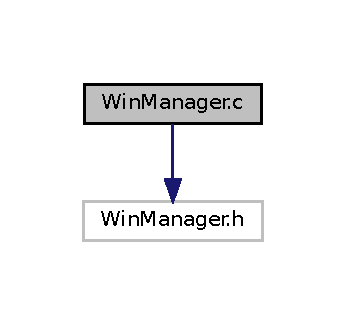
\includegraphics[width=166pt]{WinManager_8c__incl}
\end{center}
\end{figure}
\subsection*{Macros}
\begin{DoxyCompactItemize}
\item 
\#define \mbox{\hyperlink{WinManager_8c_a25f003de16c08a4888b69f619d70f427}{A\+R\+R\+A\+Y\+\_\+\+S\+I\+ZE}}(a)~(sizeof(a) / sizeof(a\mbox{[}0\mbox{]}))
\end{DoxyCompactItemize}
\subsection*{Functions}
\begin{DoxyCompactItemize}
\item 
void \mbox{\hyperlink{WinManager_8c_a849111adfa324beecdeee015db181eed}{start\+Win}} ()
\begin{DoxyCompactList}\small\item\em Função\+: Iniciar as funções da Ncurses usadas no jogo. \end{DoxyCompactList}\item 
int \mbox{\hyperlink{WinManager_8c_ab2cbbec44e25f5f9e75674f1c9a16ad1}{get\+Menu}} (int mouse\+\_\+x, int mouse\+\_\+y)
\begin{DoxyCompactList}\small\item\em Função\+: Informar a posição do cursor do mouse no menu. \end{DoxyCompactList}\item 
int \mbox{\hyperlink{WinManager_8c_adde33d501e5ef6a7d56c0a4f8ddb1dcd}{start\+Game\+Menu}} ()
\begin{DoxyCompactList}\small\item\em Função\+: Iniciar, printar e controlar o Menu do Início do Jogo. \end{DoxyCompactList}\item 
W\+I\+N\+D\+OW $\ast$ \mbox{\hyperlink{WinManager_8c_a0853f92ddde0241ba748777429c65e1c}{create\+Win}} (int Win\+Height, int Win\+Width, int Win\+Starty, int Win\+Startx)
\begin{DoxyCompactList}\small\item\em Função\+: Criar uma Janela. \end{DoxyCompactList}\item 
void \mbox{\hyperlink{WinManager_8c_adfacea1859be77ff9ae0a1224d8d88fa}{destroy\+Win}} (W\+I\+N\+D\+OW $\ast$$\ast$local\+\_\+win)
\begin{DoxyCompactList}\small\item\em Função\+: Destruir uma Janela. \end{DoxyCompactList}\item 
void \mbox{\hyperlink{WinManager_8c_af00cc56d5366ca2a981d00222dca7ccf}{middle\+Print}} (W\+I\+N\+D\+OW $\ast$win, int Win\+Starty, int Win\+Startx, int Win\+Width, char $\ast$string, chtype color)
\begin{DoxyCompactList}\small\item\em Função\+: Printa uma string em uma Janela. \end{DoxyCompactList}\item 
W\+I\+N\+D\+OW $\ast$ \mbox{\hyperlink{WinManager_8c_a6d85a472f9d03e41398d37f7a24469ee}{game\+Window}} (int win\+\_\+y, int win\+\_\+x)
\begin{DoxyCompactList}\small\item\em Função\+: Cria a Janela do Jogo. \end{DoxyCompactList}\item 
void \mbox{\hyperlink{WinManager_8c_a1f8b61e7bf767e032acd5e310ec845db}{refresh\+Windows}} (W\+I\+N\+D\+OW $\ast$\mbox{\hyperlink{GameLogic_8c_aa578a767fc3d38ab4b0211e552ed41cd}{game\+Win}}, W\+I\+N\+D\+OW $\ast$\mbox{\hyperlink{GameLogic_8c_a81cc11227a869b90adbf28221ec125a7}{status\+Win}})
\begin{DoxyCompactList}\small\item\em Função\+: Dá Refresh na Tela do jogo. \end{DoxyCompactList}\item 
void \mbox{\hyperlink{WinManager_8c_a0759424ad1942330b0dab68e64a103e9}{print\+Player\+Status}} (W\+I\+N\+D\+OW $\ast$status, Base $\ast$b, Build $\ast$b1, Build $\ast$b2, Build $\ast$b3, Troop $\ast$t1, Troop $\ast$t2, Troop $\ast$t3)
\begin{DoxyCompactList}\small\item\em Função\+: Printa os Status do Player. \end{DoxyCompactList}\item 
void \mbox{\hyperlink{WinManager_8c_aef0131e7f148c4ab7966307c5feec5a5}{print\+Enemy\+Status}} (W\+I\+N\+D\+OW $\ast$status, Base $\ast$b, Build $\ast$b1, Build $\ast$b2, Build $\ast$b3, Troop $\ast$t1, Troop $\ast$t2, Troop $\ast$t3)
\begin{DoxyCompactList}\small\item\em Função\+: Printa os Status do PC. \end{DoxyCompactList}\item 
int \mbox{\hyperlink{WinManager_8c_af61982e4a73de79a1d742ee8124e1dde}{pause\+Game\+Menu}} ()
\begin{DoxyCompactList}\small\item\em Função\+: Iniciar, printar e controlar o Menu de Pause. \end{DoxyCompactList}\item 
void \mbox{\hyperlink{WinManager_8c_a42f09a98601c46f9afd0520146181d05}{game\+End}} (Base $\ast$b\+\_\+p, Base $\ast$b\+\_\+e)
\begin{DoxyCompactList}\small\item\em Função\+: Monta e Printa uma Janela do Fim do Jogo. \end{DoxyCompactList}\end{DoxyCompactItemize}
\subsection*{Variables}
\begin{DoxyCompactItemize}
\item 
int \mbox{\hyperlink{WinManager_8c_a0d9b061718fe48dee496d1b572fa8f7b}{term\+Lines}}
\item 
int \mbox{\hyperlink{WinManager_8c_a35de4fbde28ecba7e22cb29362fdd281}{term\+Cols}}
\end{DoxyCompactItemize}


\subsection{Macro Definition Documentation}
\mbox{\Hypertarget{WinManager_8c_a25f003de16c08a4888b69f619d70f427}\label{WinManager_8c_a25f003de16c08a4888b69f619d70f427}} 
\index{Win\+Manager.\+c@{Win\+Manager.\+c}!A\+R\+R\+A\+Y\+\_\+\+S\+I\+ZE@{A\+R\+R\+A\+Y\+\_\+\+S\+I\+ZE}}
\index{A\+R\+R\+A\+Y\+\_\+\+S\+I\+ZE@{A\+R\+R\+A\+Y\+\_\+\+S\+I\+ZE}!Win\+Manager.\+c@{Win\+Manager.\+c}}
\subsubsection{\texorpdfstring{A\+R\+R\+A\+Y\+\_\+\+S\+I\+ZE}{ARRAY\_SIZE}}
{\footnotesize\ttfamily \#define A\+R\+R\+A\+Y\+\_\+\+S\+I\+ZE(\begin{DoxyParamCaption}\item[{}]{a }\end{DoxyParamCaption})~(sizeof(a) / sizeof(a\mbox{[}0\mbox{]}))}

This define gets exactly the size of the array of arrays 

\subsection{Function Documentation}
\mbox{\Hypertarget{WinManager_8c_a0853f92ddde0241ba748777429c65e1c}\label{WinManager_8c_a0853f92ddde0241ba748777429c65e1c}} 
\index{Win\+Manager.\+c@{Win\+Manager.\+c}!create\+Win@{create\+Win}}
\index{create\+Win@{create\+Win}!Win\+Manager.\+c@{Win\+Manager.\+c}}
\subsubsection{\texorpdfstring{create\+Win()}{createWin()}}
{\footnotesize\ttfamily W\+I\+N\+D\+OW$\ast$ create\+Win (\begin{DoxyParamCaption}\item[{int}]{Win\+Height,  }\item[{int}]{Win\+Width,  }\item[{int}]{Win\+Starty,  }\item[{int}]{Win\+Startx }\end{DoxyParamCaption})}



Função\+: Criar uma Janela. 

Descrição\+: A Função recebe o tamanho e uma posição no mapa e cria uma janela e retorna essa janela.

Parâmetros\+: 
\begin{DoxyParams}{Parameters}
{\em int} & Win\+Height -\/ altura da janela \\
\hline
{\em int} & Win\+Width -\/ largura da janela \\
\hline
{\em int} & Win\+Starty -\/ coordenada y que a janela vai começar a ser contruída \\
\hline
{\em int} & Win\+Startx -\/ coordenada x que a janela vai começar a ser contruída\\
\hline
\end{DoxyParams}
Valor retornado\+: \begin{DoxyReturn}{Returns}
W\+I\+N\+D\+O\+W$\ast$ local\+\_\+win -\/ janela criada
\end{DoxyReturn}
Assertiva de entrada\+: int Win\+Height $>$ 0 int Win\+Width $>$ 0 int Win\+Starty $>$= 0 int Win\+Startx $>$= 0

Assertiva de saída\+: W\+I\+N\+D\+O\+W$\ast$ local\+\_\+win != N\+U\+LL \mbox{\Hypertarget{WinManager_8c_adfacea1859be77ff9ae0a1224d8d88fa}\label{WinManager_8c_adfacea1859be77ff9ae0a1224d8d88fa}} 
\index{Win\+Manager.\+c@{Win\+Manager.\+c}!destroy\+Win@{destroy\+Win}}
\index{destroy\+Win@{destroy\+Win}!Win\+Manager.\+c@{Win\+Manager.\+c}}
\subsubsection{\texorpdfstring{destroy\+Win()}{destroyWin()}}
{\footnotesize\ttfamily void destroy\+Win (\begin{DoxyParamCaption}\item[{W\+I\+N\+D\+OW $\ast$$\ast$}]{local\+\_\+win }\end{DoxyParamCaption})}



Função\+: Destruir uma Janela. 

Descrição\+: A Função recebe uma janela e a destrói, desalocando e retirando da tela.

Parâmetros\+: 
\begin{DoxyParams}{Parameters}
{\em W\+I\+N\+D\+O\+W$\ast$$\ast$} & local\+\_\+win\\
\hline
\end{DoxyParams}
Valor retornado\+: \begin{DoxyReturn}{Returns}
Void. A função não retorna nada
\end{DoxyReturn}
Assertiva de entrada\+: W\+I\+N\+D\+O\+W$\ast$$\ast$ local\+\_\+win != N\+U\+LL

Assertiva de saída\+: Função void \mbox{\Hypertarget{WinManager_8c_a42f09a98601c46f9afd0520146181d05}\label{WinManager_8c_a42f09a98601c46f9afd0520146181d05}} 
\index{Win\+Manager.\+c@{Win\+Manager.\+c}!game\+End@{game\+End}}
\index{game\+End@{game\+End}!Win\+Manager.\+c@{Win\+Manager.\+c}}
\subsubsection{\texorpdfstring{game\+End()}{gameEnd()}}
{\footnotesize\ttfamily void game\+End (\begin{DoxyParamCaption}\item[{Base $\ast$}]{b\+\_\+p,  }\item[{Base $\ast$}]{b\+\_\+e }\end{DoxyParamCaption})}



Função\+: Monta e Printa uma Janela do Fim do Jogo. 

Descrição\+: A Função recebe as 2 structs da base (do player e do PC) e então verifica qual das duas bases tem o HP igual a 0. Se for do player é mostrada uma tela dizendo que o jogador perdeu o jogo. Se for do PC é mostrada uma tela dizendo que o jogador ganhou o jogo.

Parâmetros\+: 
\begin{DoxyParams}{Parameters}
{\em Base$\ast$} & b\+\_\+p -\/ struct da base do player \\
\hline
{\em Base$\ast$} & b\+\_\+e -\/ struct da base do PC\\
\hline
\end{DoxyParams}
Valor retornado\+: \begin{DoxyReturn}{Returns}
Void. A função apenas printa uma janela com uma mensagem
\end{DoxyReturn}
Assertiva de entrada\+: Base$\ast$ b\+\_\+p != N\+U\+LL Base$\ast$ b\+\_\+e != N\+U\+LL

Assertiva de saída\+: Função void \mbox{\Hypertarget{WinManager_8c_a6d85a472f9d03e41398d37f7a24469ee}\label{WinManager_8c_a6d85a472f9d03e41398d37f7a24469ee}} 
\index{Win\+Manager.\+c@{Win\+Manager.\+c}!game\+Window@{game\+Window}}
\index{game\+Window@{game\+Window}!Win\+Manager.\+c@{Win\+Manager.\+c}}
\subsubsection{\texorpdfstring{game\+Window()}{gameWindow()}}
{\footnotesize\ttfamily W\+I\+N\+D\+OW$\ast$ game\+Window (\begin{DoxyParamCaption}\item[{int}]{win\+\_\+y,  }\item[{int}]{win\+\_\+x }\end{DoxyParamCaption})}



Função\+: Cria a Janela do Jogo. 

Descrição\+: A Função recebe a largura e a altura de uma janela e com esses valores ela aloca e cria essa janela. Então é habilitada o keypad nessa janela. No final essa janela formada é retornada.

Parâmetros\+: 
\begin{DoxyParams}{Parameters}
{\em int} & win\+\_\+y -\/ largura da janela do jogo (número de colunas) \\
\hline
{\em int} & win\+\_\+x -\/ altura da janela do jogo (número de linhas)\\
\hline
\end{DoxyParams}
Valor retornado\+: \begin{DoxyReturn}{Returns}
W\+I\+N\+D\+O\+W$\ast$ game\+Win -\/ janela do jogo
\end{DoxyReturn}
Assertiva de entrada\+: int win\+\_\+y $>$ 0 int win\+\_\+x $>$ 0

Assertiva de saída\+: W\+I\+N\+D\+O\+W$\ast$ game\+Win != N\+U\+LL \mbox{\Hypertarget{WinManager_8c_ab2cbbec44e25f5f9e75674f1c9a16ad1}\label{WinManager_8c_ab2cbbec44e25f5f9e75674f1c9a16ad1}} 
\index{Win\+Manager.\+c@{Win\+Manager.\+c}!get\+Menu@{get\+Menu}}
\index{get\+Menu@{get\+Menu}!Win\+Manager.\+c@{Win\+Manager.\+c}}
\subsubsection{\texorpdfstring{get\+Menu()}{getMenu()}}
{\footnotesize\ttfamily int get\+Menu (\begin{DoxyParamCaption}\item[{int}]{mouse\+\_\+x,  }\item[{int}]{mouse\+\_\+y }\end{DoxyParamCaption})}



Função\+: Informar a posição do cursor do mouse no menu. 

Descrição\+: A Função recebe as coordenadas do cursor do mouse e identifica se o cursor está em algumas das opções do menu e retorna uma flag de acordo com a opção selecionada.

Parâmetros\+: 
\begin{DoxyParams}{Parameters}
{\em int} & mouse\+\_\+x -\/ posição x do cursor no menu \\
\hline
{\em int} & mouse\+\_\+y -\/ posição y do cursor no menu\\
\hline
\end{DoxyParams}
Valor retornado\+: \begin{DoxyReturn}{Returns}
int i -\/ flag que simboliza em qual opção do menu o mouse se encontra. Seus valores podem ser\+: 0 -\/ Mouse sobre nenhuma das opções 1 -\/ Mouse sobre a New Game 2 -\/ Mouse sobre o Load Game 3 -\/ Mouse sobre os Créditos 4 -\/ Mouse sobre o Exit
\end{DoxyReturn}
Assertiva de entrada\+: int mouse\+\_\+x $>$= 0 int mouse\+\_\+y $>$= 0

Assertiva de saída\+: int i == 0 $\vert$$\vert$ i == 1 $\vert$$\vert$ i == 2 $\vert$$\vert$ i == 3 $\vert$$\vert$ i == 4 \mbox{\Hypertarget{WinManager_8c_af00cc56d5366ca2a981d00222dca7ccf}\label{WinManager_8c_af00cc56d5366ca2a981d00222dca7ccf}} 
\index{Win\+Manager.\+c@{Win\+Manager.\+c}!middle\+Print@{middle\+Print}}
\index{middle\+Print@{middle\+Print}!Win\+Manager.\+c@{Win\+Manager.\+c}}
\subsubsection{\texorpdfstring{middle\+Print()}{middlePrint()}}
{\footnotesize\ttfamily void middle\+Print (\begin{DoxyParamCaption}\item[{W\+I\+N\+D\+OW $\ast$}]{win,  }\item[{int}]{Win\+Starty,  }\item[{int}]{Win\+Startx,  }\item[{int}]{Win\+Width,  }\item[{char $\ast$}]{string,  }\item[{chtype}]{color }\end{DoxyParamCaption})}



Função\+: Printa uma string em uma Janela. 

Descrição\+: A Função recebe uma janela, uma string e a cor e a posição em que essa string deve ser escrita na janela.

Parâmetros\+: 
\begin{DoxyParams}{Parameters}
{\em W\+I\+N\+D\+O\+W$\ast$} & win -\/ uma janela \\
\hline
{\em int} & Win\+Starty -\/ coordenada y que a string vai ficar \\
\hline
{\em int} & Win\+Startx -\/ coordenada x que a string vai ficar \\
\hline
{\em int} & Win\+Width -\/ largura da janela \\
\hline
{\em char$\ast$} & string -\/ string que vai ser impressa na janela \\
\hline
{\em chtype} & color -\/ cor da string\\
\hline
\end{DoxyParams}
Valor retornado\+: \begin{DoxyReturn}{Returns}
Void. A função somente imprime em uma janela
\end{DoxyReturn}
Assertiva de entrada\+: W\+I\+N\+D\+O\+W$\ast$ win != N\+U\+LL int Win\+Starty $>$= 0 int Win\+Startx $>$= 0 int Win\+Width $>$ 0 char$\ast$ string != N\+U\+LL

Assertiva de saída\+: Função Void \mbox{\Hypertarget{WinManager_8c_af61982e4a73de79a1d742ee8124e1dde}\label{WinManager_8c_af61982e4a73de79a1d742ee8124e1dde}} 
\index{Win\+Manager.\+c@{Win\+Manager.\+c}!pause\+Game\+Menu@{pause\+Game\+Menu}}
\index{pause\+Game\+Menu@{pause\+Game\+Menu}!Win\+Manager.\+c@{Win\+Manager.\+c}}
\subsubsection{\texorpdfstring{pause\+Game\+Menu()}{pauseGameMenu()}}
{\footnotesize\ttfamily int pause\+Game\+Menu (\begin{DoxyParamCaption}{ }\end{DoxyParamCaption})}



Função\+: Iniciar, printar e controlar o Menu de Pause. 

Descrição\+: A Função inicializa os itens do menu de pause, inicializa o menu, cria a janela do menu sobre a janela do jogo, printa o menu e as bordas com as suas cores. Então ela espera o usuário escolher um dos itens e dar \char`\"{}enter\char`\"{} . Depois a função destrói o menu e retorna o valor do item selecionado.

Parâmetros\+: 
\begin{DoxyParams}{Parameters}
{\em sem} & parâmetros\\
\hline
\end{DoxyParams}
Valor retornado\+: \begin{DoxyReturn}{Returns}
(long int)item\+Ptr -\/ valor do item selecionado pelo player. Dependendo da opção selecionada, a variável possui um valor. Podendo ser\+: 0 -\/ New Game 1 -\/ Load Game 2 -\/ Credits 3 -\/ Exit
\end{DoxyReturn}
Assertiva de entrada\+: sem parâmetros

Assertiva de saída\+: (long int)item\+Ptr == 0 $\vert$$\vert$ item\+Ptr == 1 $\vert$$\vert$ item\+Ptr == 2 \mbox{\Hypertarget{WinManager_8c_aef0131e7f148c4ab7966307c5feec5a5}\label{WinManager_8c_aef0131e7f148c4ab7966307c5feec5a5}} 
\index{Win\+Manager.\+c@{Win\+Manager.\+c}!print\+Enemy\+Status@{print\+Enemy\+Status}}
\index{print\+Enemy\+Status@{print\+Enemy\+Status}!Win\+Manager.\+c@{Win\+Manager.\+c}}
\subsubsection{\texorpdfstring{print\+Enemy\+Status()}{printEnemyStatus()}}
{\footnotesize\ttfamily void print\+Enemy\+Status (\begin{DoxyParamCaption}\item[{W\+I\+N\+D\+OW $\ast$}]{status,  }\item[{Base $\ast$}]{b,  }\item[{Build $\ast$}]{b1,  }\item[{Build $\ast$}]{b2,  }\item[{Build $\ast$}]{b3,  }\item[{Troop $\ast$}]{t1,  }\item[{Troop $\ast$}]{t2,  }\item[{Troop $\ast$}]{t3 }\end{DoxyParamCaption})}



Função\+: Printa os Status do PC. 

Descrição\+: A Função recebe uma janela e as structs da base, dos prédios e das tropas. Então ela printa na janela os status dessas structs, como HP, número de tropas e quantidade de recursos.

Parâmetros\+: 
\begin{DoxyParams}{Parameters}
{\em W\+I\+N\+D\+O\+W$\ast$} & status -\/ janela dos status \\
\hline
{\em Base$\ast$} & b -\/ struct da base \\
\hline
{\em Build$\ast$} & b1 -\/ struct do prédio 1 \\
\hline
{\em Build$\ast$} & b2 -\/ struct do prédio 2 \\
\hline
{\em Build$\ast$} & b3 -\/ struct do prédio 3 \\
\hline
{\em Troop$\ast$} & t1 -\/ struct da tropa 1 \\
\hline
{\em Troop$\ast$} & t2 -\/ struct da tropa 2 \\
\hline
{\em Troop$\ast$} & t3 -\/ struct da tropa 3\\
\hline
\end{DoxyParams}
Valor retornado\+: \begin{DoxyReturn}{Returns}
Void. A função apenas printa os status
\end{DoxyReturn}
Assertiva de entrada\+: W\+I\+N\+D\+O\+W$\ast$ status != N\+U\+LL Base$\ast$ b != N\+U\+LL Build$\ast$ b1 != N\+U\+LL Build$\ast$ b2 != N\+U\+LL Build$\ast$ b3 != N\+U\+LL Troop$\ast$ t1 != N\+U\+LL Troop$\ast$ t2 != N\+U\+LL Troop$\ast$ t3 != N\+U\+LL

Assertiva de saída\+: Função void \mbox{\Hypertarget{WinManager_8c_a0759424ad1942330b0dab68e64a103e9}\label{WinManager_8c_a0759424ad1942330b0dab68e64a103e9}} 
\index{Win\+Manager.\+c@{Win\+Manager.\+c}!print\+Player\+Status@{print\+Player\+Status}}
\index{print\+Player\+Status@{print\+Player\+Status}!Win\+Manager.\+c@{Win\+Manager.\+c}}
\subsubsection{\texorpdfstring{print\+Player\+Status()}{printPlayerStatus()}}
{\footnotesize\ttfamily void print\+Player\+Status (\begin{DoxyParamCaption}\item[{W\+I\+N\+D\+OW $\ast$}]{status,  }\item[{Base $\ast$}]{b,  }\item[{Build $\ast$}]{b1,  }\item[{Build $\ast$}]{b2,  }\item[{Build $\ast$}]{b3,  }\item[{Troop $\ast$}]{t1,  }\item[{Troop $\ast$}]{t2,  }\item[{Troop $\ast$}]{t3 }\end{DoxyParamCaption})}



Função\+: Printa os Status do Player. 

Descrição\+: A Função recebe uma janela e as structs da base, dos prédios e das tropas. Então ela printa na janela os status dessas structs, como HP, número de tropas e quantidade de recursos.

Parâmetros\+: 
\begin{DoxyParams}{Parameters}
{\em W\+I\+N\+D\+O\+W$\ast$} & status -\/ janela dos status \\
\hline
{\em Base$\ast$} & b -\/ struct da base \\
\hline
{\em Build$\ast$} & b1 -\/ struct do prédio 1 \\
\hline
{\em Build$\ast$} & b2 -\/ struct do prédio 2 \\
\hline
{\em Build$\ast$} & b3 -\/ struct do prédio 3 \\
\hline
{\em Troop$\ast$} & t1 -\/ struct da tropa 1 \\
\hline
{\em Troop$\ast$} & t2 -\/ struct da tropa 2 \\
\hline
{\em Troop$\ast$} & t3 -\/ struct da tropa 3\\
\hline
\end{DoxyParams}
Valor retornado\+: \begin{DoxyReturn}{Returns}
Void. A função apenas printa os status
\end{DoxyReturn}
Assertiva de entrada\+: W\+I\+N\+D\+O\+W$\ast$ status != N\+U\+LL Base$\ast$ b != N\+U\+LL Build$\ast$ b1 != N\+U\+LL Build$\ast$ b2 != N\+U\+LL Build$\ast$ b3 != N\+U\+LL Troop$\ast$ t1 != N\+U\+LL Troop$\ast$ t2 != N\+U\+LL Troop$\ast$ t3 != N\+U\+LL

Assertiva de saída\+: Função void \mbox{\Hypertarget{WinManager_8c_a1f8b61e7bf767e032acd5e310ec845db}\label{WinManager_8c_a1f8b61e7bf767e032acd5e310ec845db}} 
\index{Win\+Manager.\+c@{Win\+Manager.\+c}!refresh\+Windows@{refresh\+Windows}}
\index{refresh\+Windows@{refresh\+Windows}!Win\+Manager.\+c@{Win\+Manager.\+c}}
\subsubsection{\texorpdfstring{refresh\+Windows()}{refreshWindows()}}
{\footnotesize\ttfamily void refresh\+Windows (\begin{DoxyParamCaption}\item[{W\+I\+N\+D\+OW $\ast$}]{game\+Win,  }\item[{W\+I\+N\+D\+OW $\ast$}]{status\+Win }\end{DoxyParamCaption})}



Função\+: Dá Refresh na Tela do jogo. 

Descrição\+: A Função recebe 2 janelas, a do jogo com o mapa e a janela de status do player e PC. Então ela atualiza e dá refresh na tela de acordo com o que aconteceu dentro do jogo.

Parâmetros\+: 
\begin{DoxyParams}{Parameters}
{\em W\+I\+N\+D\+O\+W$\ast$} & game\+Win -\/ janela do jogo, onde está o mapa \\
\hline
{\em W\+I\+N\+D\+O\+W$\ast$} & status\+Win -\/ janela com os status das tropas,prédios e base do player e do PC\\
\hline
\end{DoxyParams}
Valor retornado\+: \begin{DoxyReturn}{Returns}
Void. A função apenas atualiza a tela
\end{DoxyReturn}
Assertiva de entrada\+: W\+I\+N\+D\+O\+W$\ast$ game\+Win != N\+U\+LL W\+I\+N\+D\+O\+W$\ast$ status\+Win != N\+U\+LL

Assertiva de saída\+: Função void \mbox{\Hypertarget{WinManager_8c_adde33d501e5ef6a7d56c0a4f8ddb1dcd}\label{WinManager_8c_adde33d501e5ef6a7d56c0a4f8ddb1dcd}} 
\index{Win\+Manager.\+c@{Win\+Manager.\+c}!start\+Game\+Menu@{start\+Game\+Menu}}
\index{start\+Game\+Menu@{start\+Game\+Menu}!Win\+Manager.\+c@{Win\+Manager.\+c}}
\subsubsection{\texorpdfstring{start\+Game\+Menu()}{startGameMenu()}}
{\footnotesize\ttfamily int start\+Game\+Menu (\begin{DoxyParamCaption}{ }\end{DoxyParamCaption})}



Função\+: Iniciar, printar e controlar o Menu do Início do Jogo. 

Descrição\+: A Função inicializa os itens do menu inicial, inicializa o menu, cria a janela do menu sobre a janela da ncurses, printa o menu e as bordas com as suas cores. Então ela espera o usuário escolher um dos itens e dar \char`\"{}enter\char`\"{} . Depois a função destrói o menu inicial e retorna o valor do item selecionado.

Parâmetros\+: 
\begin{DoxyParams}{Parameters}
{\em sem} & parâmetros\\
\hline
\end{DoxyParams}
Valor retornado\+: \begin{DoxyReturn}{Returns}
(long int)item\+Ptr -\/ valor do item selecionado pelo player. Dependendo da opção selecionada, a variável possui um valor. Podendo ser\+: 0 -\/ New Game 1 -\/ Load Game 2 -\/ Credits 3 -\/ Exit
\end{DoxyReturn}
Assertiva de entrada\+: sem parâmetros

Assertiva de saída\+: (long int)item\+Ptr == 0 $\vert$$\vert$ item\+Ptr == 1 $\vert$$\vert$ item\+Ptr == 2 $\vert$$\vert$ item\+Ptr == 3 \mbox{\Hypertarget{WinManager_8c_a849111adfa324beecdeee015db181eed}\label{WinManager_8c_a849111adfa324beecdeee015db181eed}} 
\index{Win\+Manager.\+c@{Win\+Manager.\+c}!start\+Win@{start\+Win}}
\index{start\+Win@{start\+Win}!Win\+Manager.\+c@{Win\+Manager.\+c}}
\subsubsection{\texorpdfstring{start\+Win()}{startWin()}}
{\footnotesize\ttfamily void start\+Win (\begin{DoxyParamCaption}{ }\end{DoxyParamCaption})}



Função\+: Iniciar as funções da Ncurses usadas no jogo. 

Descrição\+: A Função é responsável por iniciar tudo que o programa irá utilizar. Entre eles, as specials keys, as cores, o uso do mouse, captura o tamanho do terminal, desabilita o echo (a necessidade de apertar enter para capturar uma entrada) e inicia a janela da ncurses. Com tudo inicializado as outras funções podem funcionar.

Parâmetros\+: 
\begin{DoxyParams}{Parameters}
{\em sem} & parâmetros\\
\hline
\end{DoxyParams}
Valor retornado\+: \begin{DoxyReturn}{Returns}
Void -\/ a função não retorna nada
\end{DoxyReturn}
Assertiva de entrada\+: sem parâmetros

Assertiva de saída\+: função void 

\subsection{Variable Documentation}
\mbox{\Hypertarget{WinManager_8c_a35de4fbde28ecba7e22cb29362fdd281}\label{WinManager_8c_a35de4fbde28ecba7e22cb29362fdd281}} 
\index{Win\+Manager.\+c@{Win\+Manager.\+c}!term\+Cols@{term\+Cols}}
\index{term\+Cols@{term\+Cols}!Win\+Manager.\+c@{Win\+Manager.\+c}}
\subsubsection{\texorpdfstring{term\+Cols}{termCols}}
{\footnotesize\ttfamily int term\+Cols}

variável para o número de colunas do terminal \mbox{\Hypertarget{WinManager_8c_a0d9b061718fe48dee496d1b572fa8f7b}\label{WinManager_8c_a0d9b061718fe48dee496d1b572fa8f7b}} 
\index{Win\+Manager.\+c@{Win\+Manager.\+c}!term\+Lines@{term\+Lines}}
\index{term\+Lines@{term\+Lines}!Win\+Manager.\+c@{Win\+Manager.\+c}}
\subsubsection{\texorpdfstring{term\+Lines}{termLines}}
{\footnotesize\ttfamily int term\+Lines}

variável para o número de linhas do terminal 
%--- End generated contents ---

% Index
\backmatter
\newpage
\phantomsection
\clearemptydoublepage
\addcontentsline{toc}{chapter}{Index}
\printindex

\end{document}
